
\documentclass[
fontsize=12pt,
twoside=true,
a4paper,
bibliography=totoc, 		%Literaturverzeichnis ins IV
listof=totoc,				%Abb. & Tab. verz. ins IV
toc=bibliographynumbered, 	%Literaturverzeichnis im IV nummerieren
listof=numbered
]{scrreprt}

\usepackage[
a4paper,
includefoot,
includehead,
bottom=1cm, 
top=0.8cm, 
left=25mm, 
right=20mm,
twoside=false,
]{geometry}

\setlength{\footskip}{1cm}
\setlength{\textheight}{24cm}
\setlength{\headheight}{84pt}
\setlength{\headsep}{15pt}
%\usepackage[onehalfspacing]{setspace} %Zeilenabstand

%\usepackage{titlesec} 
\renewcommand*\chapterheadstartvskip{\vspace*{-1cm}}
\renewcommand*\chapterheadendvskip{\vspace*{0cm}}

% \usepackage[utf8]{inputenc} % UTF-8 als Zeichenkodierung verwenden
% \usepackage[T1]{fontenc}
\usepackage[shorthands=off,english,ngerman]{babel}
\usepackage{microtype}  % besserer Textsatz

\usepackage{enumitem} 
\usepackage{placeins}
\usepackage{longtable}
\usepackage{makeidx}
\usepackage{graphicx}
\usepackage{float}
\usepackage{fancyhdr}
\usepackage{babelbib}
\usepackage{wrapfig}
\usepackage{url}
\usepackage{totpages}
%Tabellenspalten mit fixer Groesse zentrieren
\usepackage{array}
\usepackage{multirow}
%Quellcode ordentlich anzeigen
\usepackage{listings}
%\usepackage{fontspec}


\lstdefinelanguage{JavaScript}{
  keywords={typeof, new, true, false, catch, function, return, null, catch, switch, var, if, in, while, do, else, case, break},
  keywordstyle=\color{blue}\bfseries,
  ndkeywords={class, export, boolean, throw, implements, import, this},
  ndkeywordstyle=\color{darkgray}\bfseries,
  identifierstyle=\color{black},
  sensitive=false,
  comment=[l]{//},
  morecomment=[s]{/*}{*/},
  commentstyle=\color{purple}\ttfamily,
  stringstyle=\color{red}\ttfamily,
  morestring=[b]',
  morestring=[b]"
}

\lstdefinelanguage{graphql}{
    morekeywords={query, mutation, subscription, type, input, enum, interface, union, scalar, directive, schema, extend, fragment, on, implements},
    sensitive=true,
    morecomment=[l]{\#},
    morestring=[s][\color{orange}]{""}{""},
    commentstyle=\color{purple},
    keywordstyle=\color{blue},
    stringstyle=\color{red},
    basicstyle=\ttfamily,
    breaklines,
    showstringspaces=false
}

\lstdefinelanguage{json}{
    numbers=left,
    numberstyle=\small,
    rulecolor=\color{black},
    showspaces=false,
    showtabs=false,
    breaklines=true,
    postbreak=\raisebox{0ex}[0ex][0ex]{\ensuremath{\color{gray}\hookrightarrow\space}},
    breakatwhitespace=true,
    basicstyle=\ttfamily\small,
    upquote=true,
    morestring=[b]",
    stringstyle=\color{string},
    literate=
     *{0}{{{\color{numb}0}}}{1}
      {1}{{{\color{numb}1}}}{1}
      {2}{{{\color{numb}2}}}{1}
      {3}{{{\color{numb}3}}}{1}
      {4}{{{\color{numb}4}}}{1}
      {5}{{{\color{numb}5}}}{1}
      {6}{{{\color{numb}6}}}{1}
      {7}{{{\color{numb}7}}}{1}
      {8}{{{\color{numb}8}}}{1}
      {9}{{{\color{numb}9}}}{1}
      {\{}{{{\color{delim}{\{}}}}{1}
      {\}}{{{\color{delim}{\}}}}}{1}
      {[}{{{\color{delim}{[}}}}{1}
      {]}{{{\color{delim}{]}}}}{1},
}

\lstdefinelanguage{yaml}{
    keywords={true,false,null,y,n},
    keywordstyle=\color{blue}\bfseries,
    ndkeywords={},
    ndkeywordstyle=\color{magenta}\bfseries,
    sensitive=false,
    comment=[l]{\#},
    morecomment=[s]{/*}{*/},
    commentstyle=\color{gray}\ttfamily,
    stringstyle=\color{red}\ttfamily,
    morestring=[b]',
    morestring=[b]",
    literate =
    {-}{{\textcolor{blue}{-}}}{1}
    {:}{{\textcolor{blue}{:}}}{1}, 
    tabsize=2
}


% \lstdefinelanguage{yaml}{
%    sensitive=true,
%    keywords={true,false,null,y,n},
%    % otherkeywords={:,-},
%    % literate=
%        % *{:}{{\textcolor{blue}{:}}}1
%        % {-}{{\textcolor{blue}{-}}}1
%        % {,}{{\textcolor{blue}{,}}}1
%        % {>}{{\textcolor{blue}{>}}}1
%        % {|}{{\textcolor{blue}{$\vert$}}}1
%        % {?}{\textcolor{blue}{?}}{1}
%        % {\&}{\textcolor{blue}{\&}}{1}
%        % {\*}{\textcolor{blue}{\*}}{1},
%        % {: }{{\textcolor{blue}{: }}}2,
%    morestring=[b]',
%    morestring=[b]",
%    morecomment=[l]{\#},
%    % Define keys and values
%    morekeywords=[2]{version, name, services, image, build, context, Dockerfile, hostname, ports, environment, depends_on},
%    morekeywords=[3]{true, false, null},
%    morestring=[s]{"}{"},
%    morestring=[s]{'}{'},
%    morecomment=[l]{\#},
% }

%Formatierung des Quellcodes
\usepackage{xcolor}
\usepackage{caption}
\usepackage{subcaption}
\usepackage{fontawesome5}

\usepackage{float}
\restylefloat{table}
%Standardschriftart bei Ueberschriften
\setkomafont{disposition}{\rmfamily}
%rotierte Tabellen
\usepackage{rotating} 
%PDF einfuegen
\usepackage{pdfpages}

%%%%%%%%%%%%%%%%%%%%%%%%%%%%%%%%%%%%%%%%%%%%%%%%%%%%%%%%%%%%%%%%%%%%%%%%%%%
% PDF Attribute
%
\makeatletter
\newif\ifpdfoutput
\@ifundefined{pdfoutput}
{\let\pdfoutput\@undefined}
{\ifcase\pdfoutput
  \let\pdfoutput\@undefined
  \else
  \pdfoutputtrue
  \fi
  }
\makeatother


%Hyperlinks schwarz
\usepackage[bookmarks,colorlinks=true,linkcolor=black,citecolor=black,urlcolor=black,hypertexnames=false]{hyperref}


\hypersetup{
    pdfauthor={Schneider Felix und Schlipfinger Clemens},
    pdftitle={Visualisierung der Ergebnisse des Stromnetzmodells},
    pdfsubject={Diplomarbeit},
    pdfkeywords={Apache Kafka Java GraphQL JavaScript Angular Cytoscape Fehleranalyse},
    pdfproducer={LaTeX},
    pdfcreator={LuaLaTeX}
}
  
%%%%%%%%%%%%%%%%%%%%%%%%%%%%%%%%%%%%%%%%%%%%%%%%%%%%%%%%%%%%%%%%%%%%%%%%%%%

\usepackage[
    left = \flqq{},% 
    right = \frqq{},% 
    leftsub = \flq{},% 
    rightsub = \frq{} %
]{dirtytalk}

\usepackage[skins,minted]{tcolorbox}
\tcbuselibrary{listings}

\definecolor{mintedbackground}{rgb}{0.95,0.95,0.95}

% This is the bash profile used throughout the document.
% I've also got one for Python and console text (regular commands)
\setminted[bash]{
    bgcolor=mintedbackground,
    fontfamily=tt,
    linenos=true,
    numberblanklines=true,
    numbersep=12pt,
    numbersep=5pt,
    gobble=0,
    frame=leftline,
    framesep=2mm,
    funcnamehighlighting=true,
    tabsize=4,
    obeytabs=false,
    mathescape=false
    samepage=false,
    showspaces=false,
    showtabs =false,
    texcl=false,
    baselinestretch=1.2,
    fontsize=\footnotesize,
    breaklines=true,
}

\newtcblisting{myminted}[3][]{listing engine=minted, listing only,#1, title=#2, minted language=#3, colback=mintedbackground}

%\setmonofont{JetBrains Mono}[Scale=MatchLowercase]

% Define your colors
\definecolor{codecomment}{RGB}{0,128,0}    % Green
\definecolor{codekeyword}{RGB}{0,0,255}    % Blue
\definecolor{codenumbers}{RGB}{128,128,128} % Gray
\definecolor{codestrings}{RGB}{255,0,0}    % Red

% Define your lstlisting style
\lstset{
    commentstyle=\color{codecomment},
    keywordstyle=\color{codekeyword},
    numberstyle=\tiny\color{codenumbers},
    stringstyle=\color{codestrings},
    basicstyle=\ttfamily\footnotesize,
    breakatwhitespace=false,         
    breaklines=true,                 
    captionpos=b,                    
    keepspaces=true,                 
    numbers=left,                    
    numbersep=5pt,                  
    showspaces=false,                
    showstringspaces=false,
    showtabs=false,                  
    tabsize=2
}
% \newcommand{\wordinquotes}[1]{\glq#1\grq}
\newcommand{\wordindoublequotes}[1]{\glqq#1\grqq}
%%%%%%%%%%%%%%%%%%%%%%%%%%%%%%%%%%%%%%%%%%%%%%%%%%
% 2.EINSTELLUNGEN
%%%%%%%%%%%%%%%%%%%%%%%%%%%%%%%%%%%%%%%%%%%%%%%%%%

% Indexgenerierung (Prozessoranweisung)
\makeindex

% setzt den Pfad fuer Graphiken
\graphicspath{{figures/}}
% zeigt Nummerierungen bei subsubsections an
\setcounter{secnumdepth}{4}
% Zaehler der die maximale Nummer von "Floatobjekten" am Beginn einer Seite angibt
\setcounter{topnumber}{2}
% Redefinition: gibt an, wieviel Platz Floatobjekte (Tabellen, Bilder)
% am Beginn einer Seite einnehmen duerfen. (80 Prozent)
\def\topfraction{.8}
% Zaehler der die maximale Nummer von "Floatobjekten" am Ende einer Seite angibt
\setcounter{bottomnumber}{2}
% Redefinition: gibt an, wieviel Platz Floatobjekte (Tabellen, Bilder)
% am Beginn einer Seite einnehmen duerfen. (80 Prozent)
\def\bottomfraction{.5}
% maximale Anzahl der Floatobjekte auf einer Seite
\setcounter{totalnumber}{8}
% Redefinition: minimaler Prozentsatz einer Seite der Text auf dem Text stehen muss
\def\textfraction{.2}
% Redefinition: mimimaler Prozentsatz von Floatobjekten die auf einer Floatseite(Seite,
% die nur Tabellen, Bilder enthaelt) sein muessen
\def\floatpagefraction{.6}
% Einzug des Absatzes auf 0 pt stellen
\setlength{\parindent}{0pt}
% vertikaler Zwischenraum zwischen zwei Absaetzen
\setlength{\parskip}{1ex plus 0.5ex minus 0.2ex}
% Teil des "caption" Packages: extra 20pkt links und rechts von einer Beschriftung
\setlength{\captionmargin}{20pt}
%Teil des "float" Packages
\floatstyle{plain}
% Name eines neuen "schwebenden" Objekts
\floatname{example}{Example}

\newfloat{example}{hbtp}{loe}[chapter]
\floatplacement{figure}{hbtp}
\floatplacement{table}{htbp}

% transformiert "\dollar" zum Dollarzeichen
\newcommand{\dollar}{\char36}	

% Skript fur die Abkuerzungen
% neue Umgebung mit einem Argument
\newenvironment{bfscript}[1] {
 % Liste
 \begin{list}
 % keine Eintragsmarkierung
 {}
 {\settowidth{\labelwidth}{\bf #1}
  % Abstand vom Eintrag zum linken Rand auf die Breite des Labels setzen (0, da kein Label)
  \setlength{\leftmargin}{\labelwidth}
  % das Ganze um die Abstand des Label zum Text (auch 0) danach erhoehen
  \addtolength{\leftmargin}{\labelsep}
  % Abstand der Absaetze innerhalb eines Eintrages
  \parsep 0.5ex plus 0.2ex minus 0.2ex
  % Abstand der einzelnen Einträge
  \itemsep 0.3ex
  % festlegen des Labels (fett, wenn noetig bis zum Text auffuellen)
  \renewcommand{\makelabel}[1]{\bf ##1\hfill}}}
 {\end{list}
}

%%%%%%%%%%%%%%%%%%%%%%%%%%%%%%%%%%%%%%%%%%%%%%%%%%
% 3.ABTEILUNGEN
%%%%%%%%%%%%%%%%%%%%%%%%%%%%%%%%%%%%%%%%%%%%%%%%%%

% Abteilungsregeln / Vorschriften hier eintragen !
\hyphenation{gleich-zeitig para-meter}

%%%%%%%%%%%%%%%%%%%%%%%%%%%%%%%%%%%%%%%%%%%%%%%%%%
% 4.ANFANG des DOKUMENTES
%%%%%%%%%%%%%%%%%%%%%%%%%%%%%%%%%%%%%%%%%%%%%%%%%%
\begin{document}
%============================================== %
% definiert das Aussehen der Kopf und Fusszeilen
\pagestyle{fancy} %eigener Seitenstil
\fancyhf{} %alle Kopf- und Fusszeilenfelder bereinigen

\chead{
\begin{tabular}{| >{\centering\arraybackslash}m{3.5cm} | p{4.5cm} p{7.65cm}|}
\hline
  \rule{0pt}{4ex} %vertikaler Abstand
  \multirow{2.5}{*}{
\includegraphics[width=2.87cm]{figures/krems.pdf}} & 
  \multicolumn{2}{c|}{\textbf{HÖHERE TECHNISCHE BUNDES - LEHRANSTALT}} \\[-0.1cm]  & \multicolumn{2}{c|}{\textbf{Krems}} \\
  \cline{2-3} \rule{0pt}{2.8ex}
    & Abteilung: & \textbf{Informationstechnologie} \\ % [-0.1cm]
    & Ausbildungsschwerpunkt: &  \\      
\hline
\end{tabular}
}

% \chead{
% \begin{tabular}{| >{\centering\arraybackslash}m{3.5cm} | p{4.5cm} p{7.65cm}|}
% \hline
%   \rule{0pt}{4ex} %vertikaler Abstand
%   \multirow{-1.5}{*}{
\includegraphics[width=2.87cm]{figures/krems.pdf}} & 
%   \multicolumn{2}{c|}{\textbf{HÖHERE TECHNISCHE BUNDES - LEHRANSTALT}} \\[-0.1cm]  & \multicolumn{2}{c|}{\textbf{Krems}} \\
%   \cline{2-3} \rule{0pt}{2.8ex}
%     & Abteilung: & \textbf{Informationstechnologie} \\ % [-0.1cm]
%     % & Ausbildungsschwerpunkt: &  \\      
% \hline
% \end{tabular}
% }

\fancyfoot[R]{Seite \thepage{} von \ref{TotPages}} %Fußzeile Seitenzahl
\renewcommand*{\chapterpagestyle}{fancy} %auch Kapitelseiten haben
\renewcommand{\headrulewidth}{0pt} %Linie unter Kopfzeile entfernen
\setcounter{page}{2} %Pagecounter bei 2 beginnen lassen (wegen Titelblatt)
%============================================== %

%benennt Quellcodelistings von "Listing" auf "Quellcode" um
\renewcommand*\lstlistingname{Quellcode}
\pagenumbering{arabic}

\definecolor{delim}{RGB}{20,105,176}
\definecolor{numb}{RGB}{21,150,135}
\definecolor{string}{rgb}{0.64,0.08,0.08}
\chapter{Einleitung}
\label{chp:introduction}
\section{Ausgangssituation und Problemstellung}

Das Unternehmen Siemens entwickelt für viele Kunden innerhalb und außerhalb von Österreich ein System, welches die Ausfallsicherheit des Stromnetzwerkes ständig überprüft und somit garantiert. Diese Software trägt den Namen \emph{Siemens GNA}. Aufgrund der unzähligen Elemente, wie zum Beispiel Sammelschienen, Ableiter, Generatoren, Transformatoren, Trennschalter, Leistungsschalter, Stationen, Sicherungen und Lasttrennschalter, besteht dieses Stromnetzwerk aus äußerst komplexen Daten. Außerdem kann es bei so vielen Elementen leicht passieren, dass gewisse Fehler, meistens in Form von Abweichungen von Sollwerten, im Netzmodell auftreten. Diese Fehler werden von Siemens erfasst, jedoch wird aktuell über keine Applikation verfügt, welche diese gefundenen Fehlerdaten effizient verarbeitet und visualisiert. Die Ingenieure bei Siemens analysieren die Fehler mittels einfachen Textdateien, welche nur schwer lesbar sind und bei einem groben Ausfall die Dauer der Reparatur unnötig vergrößern.

Um die Analyse der Fehlerdaten effizienter zu machen, schreiben Clemens Schlipfinger und Felix Schneider eine Applikation, welche diese stark vernetzten Daten mit optimalen Darstellungsarten visualisiert. Dabei gehen wir in dieser Arbeit besonders auf die Gestaltung eines entkoppelten Backend-Systems und einige geeigneten Visualisierungsarten für solch komplexe Daten ein. 

In der Abbildung \ref{fig:architecture_einleitung} wird die Architektur unserer Applikation zur Fehlervisualisierung dargestellt. Die Fehlerdaten werden von der Siemens GNA Software (\emph{Global Network Analysis} erzeugt und mittels Apache Kafka an das Backend-System übertragen. Damit wird eine hohe Entkoppelung zwischen der Siemens Software und unserem System erreicht. Für die Entwicklung und die Verwaltung von beiden Systemen ist eine hohe Unabhängigkeit von großem Wert. Anschließend werden diese Daten in eine PostgreSQL Datenbank gespeichert und mit einer GraphQL API zur Verfügung gestellt. Das Frontend, welches mit dem JavaScript Framework Angular entwickelt worden ist, wird mit Tabellen und Graphen die Fehler visualisieren.  

\begin{figure}
    \centering
    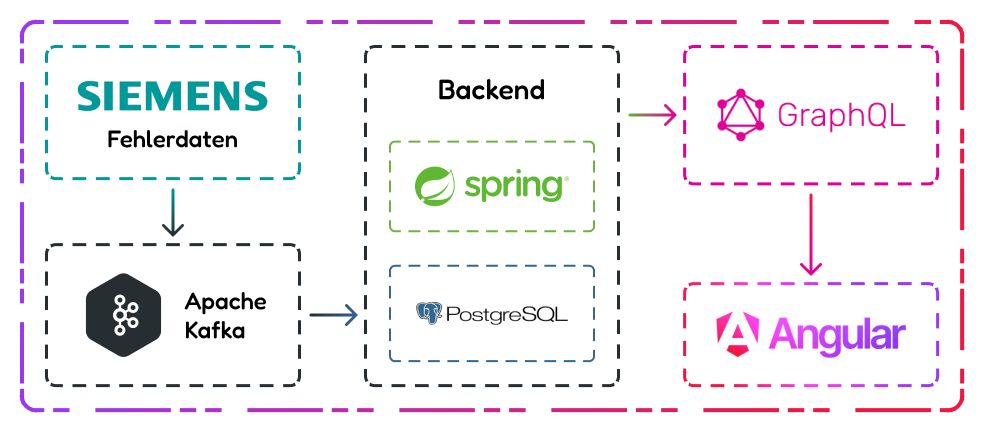
\includegraphics[width=0.8\textwidth]{content/img/Architecture/Architecture.jpg}
    \caption{Diese Darstellung zeigt den schematischen Aufbau der Applikation.}
    \label{fig:architecture_einleitung}
\end{figure}
\FloatBarrier
\section{Initial situation and problem definition}

The company Siemens develops a system called Siemens GNA for many customers both within and outside of Austria, which constantly monitors and guarantees the reliability of the power grid. Due to the numerous elements such as busbars, surge arresters, generators, transformers, disconnectors, circuit breakers, stations, fuses, and load break switches, this utility grid consists of highly complex data. Additionally, with so many elements, it is easy for certain errors, usually in the form of deviations from set values, to occur in the network model. These errors are detected by Siemens, but currently, there is no application available to efficiently process and visualize these collected error data.

Engineers at Siemens analyze the errors using simple text files, which are difficult to read and unnecessarily prolong the duration of repair in the event of a major outage. To make the analysis of error data more efficient, Clemens Schlipfinger and Felix Schneider are developing an application that visualizes these interconnected data with optimal visualization methods. In this work, they focus particularly on the design of a decoupled backend system, which is implemented in the prototype using Apache Kafka, and some suitable visualization methods for such complex data.

As you can see, the illustration \ref{fig:architecture_introduction} visualizes the architecture of our system. First, the fault data is generated by a piece of software from Siemens, which is called GNA (\emph{Global Network Analysis}) and transported to the backend over a fail-safe Apache Kafka system. This message bus decouples our system and the software from Siemens even more and enhances the reliability. Subsequently, the data is saved into a relational database called PostgreSQL. The GraphQL API provides an interface for the frontend application, which is based on the JavaScript-Framework Angular. The frontend offers great visualizations and filters in order to provide intuitive information.

\begin{figure}
    \centering
    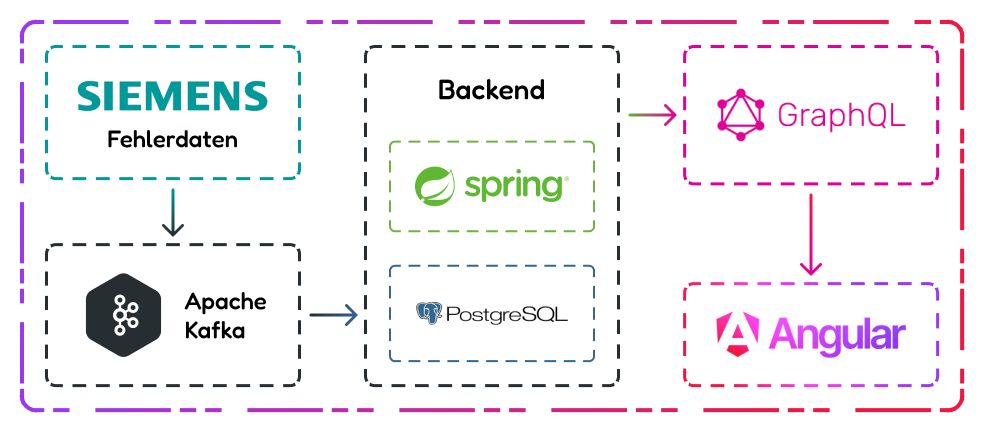
\includegraphics[width=0.8\textwidth]{content/img/Architecture/Architecture.jpg}
    \caption{This illustration shows the architecture of our application.}
    \label{fig:architecture_introduction}
\end{figure}
\FloatBarrier
\section{Forschungsfragen}

\subsection{Message Propagation}

Heutzutage ist die Ausfallsicherheit moderner Systeme von höchster Wichtigkeit. Entkoppelte Systeme fördern die Last, unter welcher Applikationen operieren können. Ein Service ist mit anderen niedrig gekoppelt, wenn wenig Abhängigkeiten gegeben sind. Die Messagepropagation unterstützt ein System dahingehend, die Kommunikation zwischen den einzelnen Softwarekomponenten in ein eigenes Service auszulagern. Welche Form der Messagepropagation am besten für verschiedene Anwendungszwecke geeignet ist, ist demnach eine Frage von hoher Bedeutung.

Demnach wird folgendes Gebiet erforscht:

\textit{Vergleich der verschiedenen Formen der Messagepropagation in Enterprise Service Bus Technologien}

\subsection{Optimale Darstellungsmethoden}

Soziale Netzwerke, biologische Systeme, Nahrungsketten, Dateisysteme und viele weitere Vorkommnisse stark vernetzter Daten verlangen eine effiziente Visualisierung dieser Datenflut. Vernetzungen dieser Art können in den meisten Fällen in gigantischen Graphen dargestellt werden, jedoch können daraus keine Informationen für das Treffen relevanter Entscheidungen getroffen werden. Wie komplexe Daten deswegen intuitiv und verständlich dargestellt werden, ist eine essenzielle Frage bei der Entwicklung solcher Systeme.

Daraus ergibt sich folgende Forschungsfrage:

\textit{Visualisierungsmethoden für stark vernetzte Daten}
\section{Strukturierung der Arbeit}

Der Inhalt dieser Arbeit unterteilt sich in drei Hauptabschnitte. Jedes dieser Kapitel kann eindeutig einem Abschnitt zugeordnet werden. Die Hauptabschnitte beschäftigen sich in erster Linie mit dem Sammeln aller aktuell vorhandenen Informationen zu den jeweiligen Themen, bekannt als \emph{State of the Art} oder \emph{Research}. Um mit der Materie vertraut zu werden, sind bestehende Forschungen der Literatur zusammengetragen und aufgearbeitet worden. Anschließend folgt der empirische Teil mit den Erklärungen der Implementierung des Prototypens, welcher zum Beweisen der These herangezogen wird, und schlussendlich die Bewertung der Forschungsfragen. Letzteres inkludiert einen Katalog zur Bestimmung der richtigen Form von Message Propagation und Vor- und Nachteile der verschiedenen Visualisierungsmethoden bei stark vernetzten Daten.
%erstellt das Inhaltsverzeichnis
\tableofcontents
\chapter{Einleitung}
\label{chp:introduction}
\section{Ausgangssituation und Problemstellung}

Das Unternehmen Siemens entwickelt für viele Kunden innerhalb und außerhalb von Österreich ein System, welches die Ausfallsicherheit des Stromnetzwerkes ständig überprüft und somit garantiert. Diese Software trägt den Namen \emph{Siemens GNA}. Aufgrund der unzähligen Elemente, wie zum Beispiel Sammelschienen, Ableiter, Generatoren, Transformatoren, Trennschalter, Leistungsschalter, Stationen, Sicherungen und Lasttrennschalter, besteht dieses Stromnetzwerk aus äußerst komplexen Daten. Außerdem kann es bei so vielen Elementen leicht passieren, dass gewisse Fehler, meistens in Form von Abweichungen von Sollwerten, im Netzmodell auftreten. Diese Fehler werden von Siemens erfasst, jedoch wird aktuell über keine Applikation verfügt, welche diese gefundenen Fehlerdaten effizient verarbeitet und visualisiert. Die Ingenieure bei Siemens analysieren die Fehler mittels einfachen Textdateien, welche nur schwer lesbar sind und bei einem groben Ausfall die Dauer der Reparatur unnötig vergrößern.

Um die Analyse der Fehlerdaten effizienter zu machen, schreiben Clemens Schlipfinger und Felix Schneider eine Applikation, welche diese stark vernetzten Daten mit optimalen Darstellungsarten visualisiert. Dabei gehen wir in dieser Arbeit besonders auf die Gestaltung eines entkoppelten Backend-Systems und einige geeigneten Visualisierungsarten für solch komplexe Daten ein. 

In der Abbildung \ref{fig:architecture_einleitung} wird die Architektur unserer Applikation zur Fehlervisualisierung dargestellt. Die Fehlerdaten werden von der Siemens GNA Software (\emph{Global Network Analysis} erzeugt und mittels Apache Kafka an das Backend-System übertragen. Damit wird eine hohe Entkoppelung zwischen der Siemens Software und unserem System erreicht. Für die Entwicklung und die Verwaltung von beiden Systemen ist eine hohe Unabhängigkeit von großem Wert. Anschließend werden diese Daten in eine PostgreSQL Datenbank gespeichert und mit einer GraphQL API zur Verfügung gestellt. Das Frontend, welches mit dem JavaScript Framework Angular entwickelt worden ist, wird mit Tabellen und Graphen die Fehler visualisieren.  

\begin{figure}
    \centering
    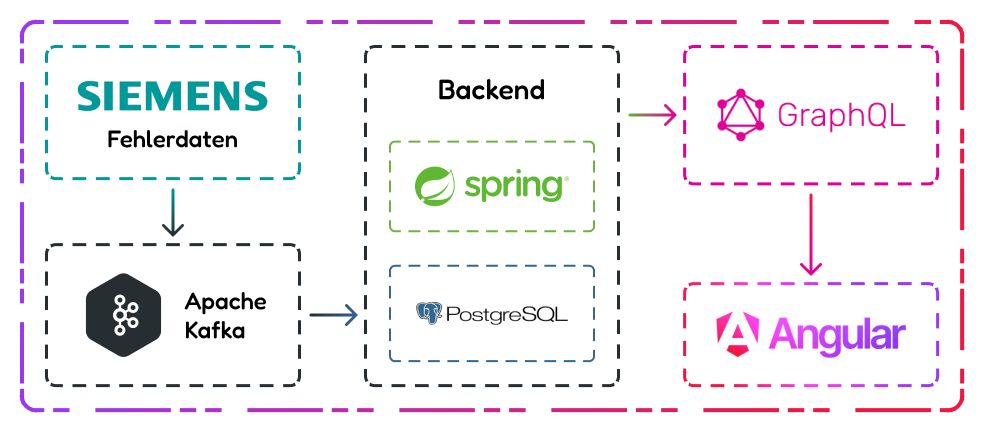
\includegraphics[width=0.8\textwidth]{content/img/Architecture/Architecture.jpg}
    \caption{Diese Darstellung zeigt den schematischen Aufbau der Applikation.}
    \label{fig:architecture_einleitung}
\end{figure}
\FloatBarrier
\section{Initial situation and problem definition}

The company Siemens develops a system called Siemens GNA for many customers both within and outside of Austria, which constantly monitors and guarantees the reliability of the power grid. Due to the numerous elements such as busbars, surge arresters, generators, transformers, disconnectors, circuit breakers, stations, fuses, and load break switches, this utility grid consists of highly complex data. Additionally, with so many elements, it is easy for certain errors, usually in the form of deviations from set values, to occur in the network model. These errors are detected by Siemens, but currently, there is no application available to efficiently process and visualize these collected error data.

Engineers at Siemens analyze the errors using simple text files, which are difficult to read and unnecessarily prolong the duration of repair in the event of a major outage. To make the analysis of error data more efficient, Clemens Schlipfinger and Felix Schneider are developing an application that visualizes these interconnected data with optimal visualization methods. In this work, they focus particularly on the design of a decoupled backend system, which is implemented in the prototype using Apache Kafka, and some suitable visualization methods for such complex data.

As you can see, the illustration \ref{fig:architecture_introduction} visualizes the architecture of our system. First, the fault data is generated by a piece of software from Siemens, which is called GNA (\emph{Global Network Analysis}) and transported to the backend over a fail-safe Apache Kafka system. This message bus decouples our system and the software from Siemens even more and enhances the reliability. Subsequently, the data is saved into a relational database called PostgreSQL. The GraphQL API provides an interface for the frontend application, which is based on the JavaScript-Framework Angular. The frontend offers great visualizations and filters in order to provide intuitive information.

\begin{figure}
    \centering
    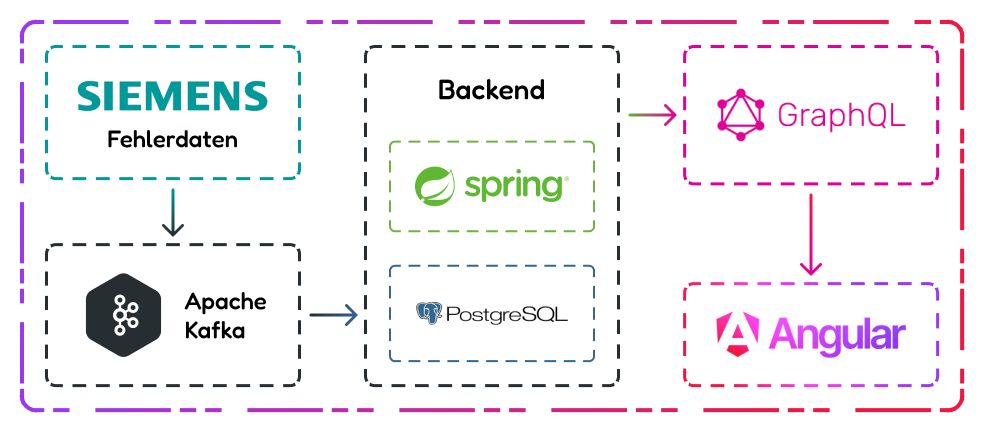
\includegraphics[width=0.8\textwidth]{content/img/Architecture/Architecture.jpg}
    \caption{This illustration shows the architecture of our application.}
    \label{fig:architecture_introduction}
\end{figure}
\FloatBarrier
\section{Forschungsfragen}

\subsection{Message Propagation}

Heutzutage ist die Ausfallsicherheit moderner Systeme von höchster Wichtigkeit. Entkoppelte Systeme fördern die Last, unter welcher Applikationen operieren können. Ein Service ist mit anderen niedrig gekoppelt, wenn wenig Abhängigkeiten gegeben sind. Die Messagepropagation unterstützt ein System dahingehend, die Kommunikation zwischen den einzelnen Softwarekomponenten in ein eigenes Service auszulagern. Welche Form der Messagepropagation am besten für verschiedene Anwendungszwecke geeignet ist, ist demnach eine Frage von hoher Bedeutung.

Demnach wird folgendes Gebiet erforscht:

\textit{Vergleich der verschiedenen Formen der Messagepropagation in Enterprise Service Bus Technologien}

\subsection{Optimale Darstellungsmethoden}

Soziale Netzwerke, biologische Systeme, Nahrungsketten, Dateisysteme und viele weitere Vorkommnisse stark vernetzter Daten verlangen eine effiziente Visualisierung dieser Datenflut. Vernetzungen dieser Art können in den meisten Fällen in gigantischen Graphen dargestellt werden, jedoch können daraus keine Informationen für das Treffen relevanter Entscheidungen getroffen werden. Wie komplexe Daten deswegen intuitiv und verständlich dargestellt werden, ist eine essenzielle Frage bei der Entwicklung solcher Systeme.

Daraus ergibt sich folgende Forschungsfrage:

\textit{Visualisierungsmethoden für stark vernetzte Daten}
\section{Strukturierung der Arbeit}

Der Inhalt dieser Arbeit unterteilt sich in drei Hauptabschnitte. Jedes dieser Kapitel kann eindeutig einem Abschnitt zugeordnet werden. Die Hauptabschnitte beschäftigen sich in erster Linie mit dem Sammeln aller aktuell vorhandenen Informationen zu den jeweiligen Themen, bekannt als \emph{State of the Art} oder \emph{Research}. Um mit der Materie vertraut zu werden, sind bestehende Forschungen der Literatur zusammengetragen und aufgearbeitet worden. Anschließend folgt der empirische Teil mit den Erklärungen der Implementierung des Prototypens, welcher zum Beweisen der These herangezogen wird, und schlussendlich die Bewertung der Forschungsfragen. Letzteres inkludiert einen Katalog zur Bestimmung der richtigen Form von Message Propagation und Vor- und Nachteile der verschiedenen Visualisierungsmethoden bei stark vernetzten Daten.
\chapter{Einleitung}
\label{chp:introduction}
\section{Ausgangssituation und Problemstellung}

Das Unternehmen Siemens entwickelt für viele Kunden innerhalb und außerhalb von Österreich ein System, welches die Ausfallsicherheit des Stromnetzwerkes ständig überprüft und somit garantiert. Diese Software trägt den Namen \emph{Siemens GNA}. Aufgrund der unzähligen Elemente, wie zum Beispiel Sammelschienen, Ableiter, Generatoren, Transformatoren, Trennschalter, Leistungsschalter, Stationen, Sicherungen und Lasttrennschalter, besteht dieses Stromnetzwerk aus äußerst komplexen Daten. Außerdem kann es bei so vielen Elementen leicht passieren, dass gewisse Fehler, meistens in Form von Abweichungen von Sollwerten, im Netzmodell auftreten. Diese Fehler werden von Siemens erfasst, jedoch wird aktuell über keine Applikation verfügt, welche diese gefundenen Fehlerdaten effizient verarbeitet und visualisiert. Die Ingenieure bei Siemens analysieren die Fehler mittels einfachen Textdateien, welche nur schwer lesbar sind und bei einem groben Ausfall die Dauer der Reparatur unnötig vergrößern.

Um die Analyse der Fehlerdaten effizienter zu machen, schreiben Clemens Schlipfinger und Felix Schneider eine Applikation, welche diese stark vernetzten Daten mit optimalen Darstellungsarten visualisiert. Dabei gehen wir in dieser Arbeit besonders auf die Gestaltung eines entkoppelten Backend-Systems und einige geeigneten Visualisierungsarten für solch komplexe Daten ein. 

In der Abbildung \ref{fig:architecture_einleitung} wird die Architektur unserer Applikation zur Fehlervisualisierung dargestellt. Die Fehlerdaten werden von der Siemens GNA Software (\emph{Global Network Analysis} erzeugt und mittels Apache Kafka an das Backend-System übertragen. Damit wird eine hohe Entkoppelung zwischen der Siemens Software und unserem System erreicht. Für die Entwicklung und die Verwaltung von beiden Systemen ist eine hohe Unabhängigkeit von großem Wert. Anschließend werden diese Daten in eine PostgreSQL Datenbank gespeichert und mit einer GraphQL API zur Verfügung gestellt. Das Frontend, welches mit dem JavaScript Framework Angular entwickelt worden ist, wird mit Tabellen und Graphen die Fehler visualisieren.  

\begin{figure}
    \centering
    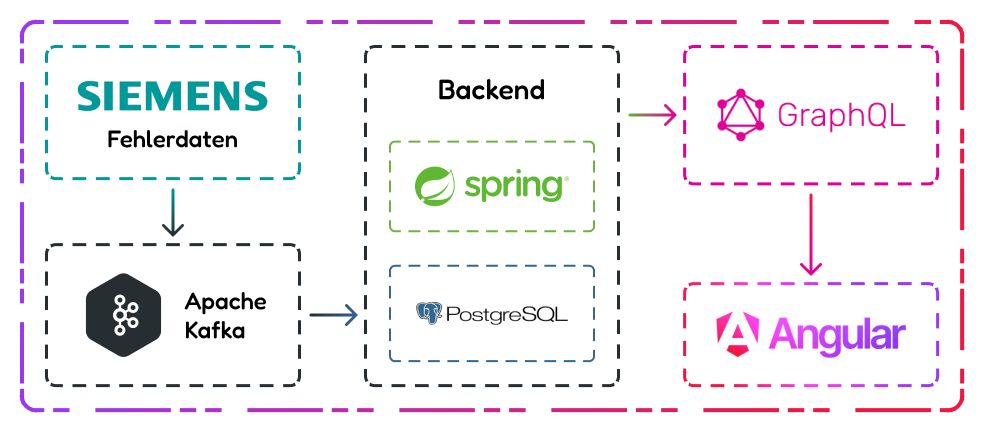
\includegraphics[width=0.8\textwidth]{content/img/Architecture/Architecture.jpg}
    \caption{Diese Darstellung zeigt den schematischen Aufbau der Applikation.}
    \label{fig:architecture_einleitung}
\end{figure}
\FloatBarrier
\section{Initial situation and problem definition}

The company Siemens develops a system called Siemens GNA for many customers both within and outside of Austria, which constantly monitors and guarantees the reliability of the power grid. Due to the numerous elements such as busbars, surge arresters, generators, transformers, disconnectors, circuit breakers, stations, fuses, and load break switches, this utility grid consists of highly complex data. Additionally, with so many elements, it is easy for certain errors, usually in the form of deviations from set values, to occur in the network model. These errors are detected by Siemens, but currently, there is no application available to efficiently process and visualize these collected error data.

Engineers at Siemens analyze the errors using simple text files, which are difficult to read and unnecessarily prolong the duration of repair in the event of a major outage. To make the analysis of error data more efficient, Clemens Schlipfinger and Felix Schneider are developing an application that visualizes these interconnected data with optimal visualization methods. In this work, they focus particularly on the design of a decoupled backend system, which is implemented in the prototype using Apache Kafka, and some suitable visualization methods for such complex data.

As you can see, the illustration \ref{fig:architecture_introduction} visualizes the architecture of our system. First, the fault data is generated by a piece of software from Siemens, which is called GNA (\emph{Global Network Analysis}) and transported to the backend over a fail-safe Apache Kafka system. This message bus decouples our system and the software from Siemens even more and enhances the reliability. Subsequently, the data is saved into a relational database called PostgreSQL. The GraphQL API provides an interface for the frontend application, which is based on the JavaScript-Framework Angular. The frontend offers great visualizations and filters in order to provide intuitive information.

\begin{figure}
    \centering
    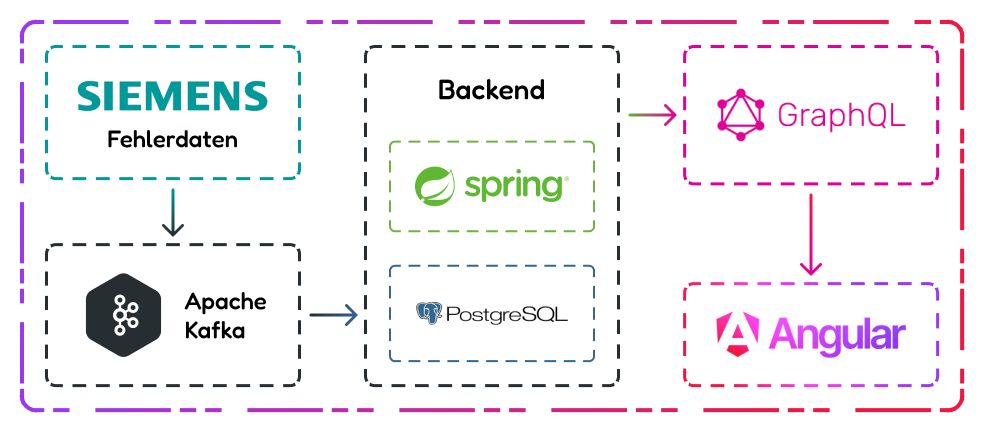
\includegraphics[width=0.8\textwidth]{content/img/Architecture/Architecture.jpg}
    \caption{This illustration shows the architecture of our application.}
    \label{fig:architecture_introduction}
\end{figure}
\FloatBarrier
\section{Forschungsfragen}

\subsection{Message Propagation}

Heutzutage ist die Ausfallsicherheit moderner Systeme von höchster Wichtigkeit. Entkoppelte Systeme fördern die Last, unter welcher Applikationen operieren können. Ein Service ist mit anderen niedrig gekoppelt, wenn wenig Abhängigkeiten gegeben sind. Die Messagepropagation unterstützt ein System dahingehend, die Kommunikation zwischen den einzelnen Softwarekomponenten in ein eigenes Service auszulagern. Welche Form der Messagepropagation am besten für verschiedene Anwendungszwecke geeignet ist, ist demnach eine Frage von hoher Bedeutung.

Demnach wird folgendes Gebiet erforscht:

\textit{Vergleich der verschiedenen Formen der Messagepropagation in Enterprise Service Bus Technologien}

\subsection{Optimale Darstellungsmethoden}

Soziale Netzwerke, biologische Systeme, Nahrungsketten, Dateisysteme und viele weitere Vorkommnisse stark vernetzter Daten verlangen eine effiziente Visualisierung dieser Datenflut. Vernetzungen dieser Art können in den meisten Fällen in gigantischen Graphen dargestellt werden, jedoch können daraus keine Informationen für das Treffen relevanter Entscheidungen getroffen werden. Wie komplexe Daten deswegen intuitiv und verständlich dargestellt werden, ist eine essenzielle Frage bei der Entwicklung solcher Systeme.

Daraus ergibt sich folgende Forschungsfrage:

\textit{Visualisierungsmethoden für stark vernetzte Daten}
\section{Strukturierung der Arbeit}

Der Inhalt dieser Arbeit unterteilt sich in drei Hauptabschnitte. Jedes dieser Kapitel kann eindeutig einem Abschnitt zugeordnet werden. Die Hauptabschnitte beschäftigen sich in erster Linie mit dem Sammeln aller aktuell vorhandenen Informationen zu den jeweiligen Themen, bekannt als \emph{State of the Art} oder \emph{Research}. Um mit der Materie vertraut zu werden, sind bestehende Forschungen der Literatur zusammengetragen und aufgearbeitet worden. Anschließend folgt der empirische Teil mit den Erklärungen der Implementierung des Prototypens, welcher zum Beweisen der These herangezogen wird, und schlussendlich die Bewertung der Forschungsfragen. Letzteres inkludiert einen Katalog zur Bestimmung der richtigen Form von Message Propagation und Vor- und Nachteile der verschiedenen Visualisierungsmethoden bei stark vernetzten Daten.
\chapter{Einleitung}
\label{chp:introduction}
\section{Ausgangssituation und Problemstellung}

Das Unternehmen Siemens entwickelt für viele Kunden innerhalb und außerhalb von Österreich ein System, welches die Ausfallsicherheit des Stromnetzwerkes ständig überprüft und somit garantiert. Diese Software trägt den Namen \emph{Siemens GNA}. Aufgrund der unzähligen Elemente, wie zum Beispiel Sammelschienen, Ableiter, Generatoren, Transformatoren, Trennschalter, Leistungsschalter, Stationen, Sicherungen und Lasttrennschalter, besteht dieses Stromnetzwerk aus äußerst komplexen Daten. Außerdem kann es bei so vielen Elementen leicht passieren, dass gewisse Fehler, meistens in Form von Abweichungen von Sollwerten, im Netzmodell auftreten. Diese Fehler werden von Siemens erfasst, jedoch wird aktuell über keine Applikation verfügt, welche diese gefundenen Fehlerdaten effizient verarbeitet und visualisiert. Die Ingenieure bei Siemens analysieren die Fehler mittels einfachen Textdateien, welche nur schwer lesbar sind und bei einem groben Ausfall die Dauer der Reparatur unnötig vergrößern.

Um die Analyse der Fehlerdaten effizienter zu machen, schreiben Clemens Schlipfinger und Felix Schneider eine Applikation, welche diese stark vernetzten Daten mit optimalen Darstellungsarten visualisiert. Dabei gehen wir in dieser Arbeit besonders auf die Gestaltung eines entkoppelten Backend-Systems und einige geeigneten Visualisierungsarten für solch komplexe Daten ein. 

In der Abbildung \ref{fig:architecture_einleitung} wird die Architektur unserer Applikation zur Fehlervisualisierung dargestellt. Die Fehlerdaten werden von der Siemens GNA Software (\emph{Global Network Analysis} erzeugt und mittels Apache Kafka an das Backend-System übertragen. Damit wird eine hohe Entkoppelung zwischen der Siemens Software und unserem System erreicht. Für die Entwicklung und die Verwaltung von beiden Systemen ist eine hohe Unabhängigkeit von großem Wert. Anschließend werden diese Daten in eine PostgreSQL Datenbank gespeichert und mit einer GraphQL API zur Verfügung gestellt. Das Frontend, welches mit dem JavaScript Framework Angular entwickelt worden ist, wird mit Tabellen und Graphen die Fehler visualisieren.  

\begin{figure}
    \centering
    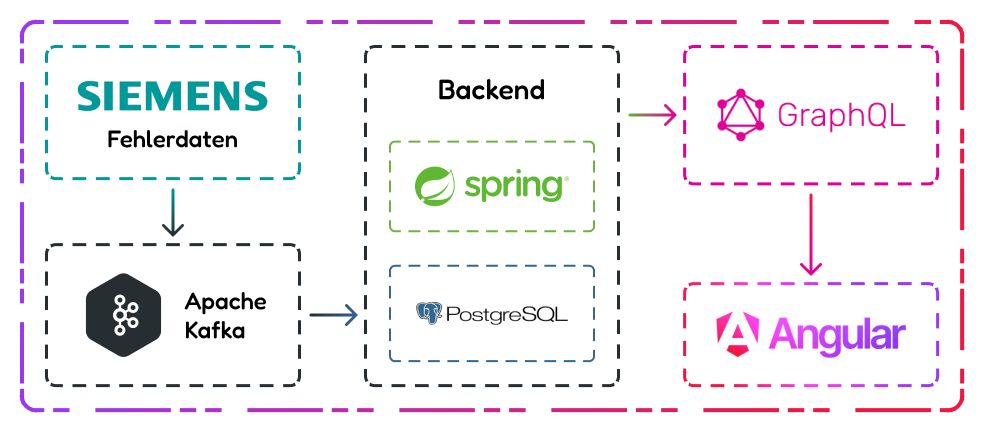
\includegraphics[width=0.8\textwidth]{content/img/Architecture/Architecture.jpg}
    \caption{Diese Darstellung zeigt den schematischen Aufbau der Applikation.}
    \label{fig:architecture_einleitung}
\end{figure}
\FloatBarrier
\section{Initial situation and problem definition}

The company Siemens develops a system called Siemens GNA for many customers both within and outside of Austria, which constantly monitors and guarantees the reliability of the power grid. Due to the numerous elements such as busbars, surge arresters, generators, transformers, disconnectors, circuit breakers, stations, fuses, and load break switches, this utility grid consists of highly complex data. Additionally, with so many elements, it is easy for certain errors, usually in the form of deviations from set values, to occur in the network model. These errors are detected by Siemens, but currently, there is no application available to efficiently process and visualize these collected error data.

Engineers at Siemens analyze the errors using simple text files, which are difficult to read and unnecessarily prolong the duration of repair in the event of a major outage. To make the analysis of error data more efficient, Clemens Schlipfinger and Felix Schneider are developing an application that visualizes these interconnected data with optimal visualization methods. In this work, they focus particularly on the design of a decoupled backend system, which is implemented in the prototype using Apache Kafka, and some suitable visualization methods for such complex data.

As you can see, the illustration \ref{fig:architecture_introduction} visualizes the architecture of our system. First, the fault data is generated by a piece of software from Siemens, which is called GNA (\emph{Global Network Analysis}) and transported to the backend over a fail-safe Apache Kafka system. This message bus decouples our system and the software from Siemens even more and enhances the reliability. Subsequently, the data is saved into a relational database called PostgreSQL. The GraphQL API provides an interface for the frontend application, which is based on the JavaScript-Framework Angular. The frontend offers great visualizations and filters in order to provide intuitive information.

\begin{figure}
    \centering
    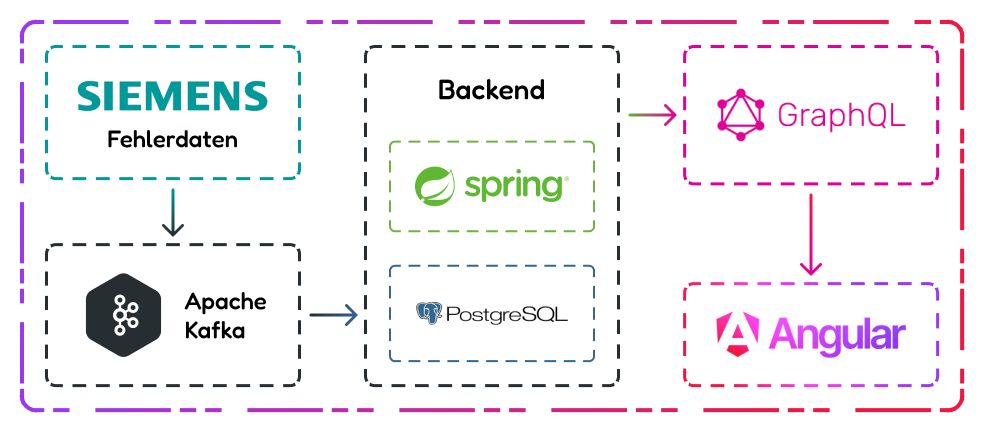
\includegraphics[width=0.8\textwidth]{content/img/Architecture/Architecture.jpg}
    \caption{This illustration shows the architecture of our application.}
    \label{fig:architecture_introduction}
\end{figure}
\FloatBarrier
\section{Forschungsfragen}

\subsection{Message Propagation}

Heutzutage ist die Ausfallsicherheit moderner Systeme von höchster Wichtigkeit. Entkoppelte Systeme fördern die Last, unter welcher Applikationen operieren können. Ein Service ist mit anderen niedrig gekoppelt, wenn wenig Abhängigkeiten gegeben sind. Die Messagepropagation unterstützt ein System dahingehend, die Kommunikation zwischen den einzelnen Softwarekomponenten in ein eigenes Service auszulagern. Welche Form der Messagepropagation am besten für verschiedene Anwendungszwecke geeignet ist, ist demnach eine Frage von hoher Bedeutung.

Demnach wird folgendes Gebiet erforscht:

\textit{Vergleich der verschiedenen Formen der Messagepropagation in Enterprise Service Bus Technologien}

\subsection{Optimale Darstellungsmethoden}

Soziale Netzwerke, biologische Systeme, Nahrungsketten, Dateisysteme und viele weitere Vorkommnisse stark vernetzter Daten verlangen eine effiziente Visualisierung dieser Datenflut. Vernetzungen dieser Art können in den meisten Fällen in gigantischen Graphen dargestellt werden, jedoch können daraus keine Informationen für das Treffen relevanter Entscheidungen getroffen werden. Wie komplexe Daten deswegen intuitiv und verständlich dargestellt werden, ist eine essenzielle Frage bei der Entwicklung solcher Systeme.

Daraus ergibt sich folgende Forschungsfrage:

\textit{Visualisierungsmethoden für stark vernetzte Daten}
\section{Strukturierung der Arbeit}

Der Inhalt dieser Arbeit unterteilt sich in drei Hauptabschnitte. Jedes dieser Kapitel kann eindeutig einem Abschnitt zugeordnet werden. Die Hauptabschnitte beschäftigen sich in erster Linie mit dem Sammeln aller aktuell vorhandenen Informationen zu den jeweiligen Themen, bekannt als \emph{State of the Art} oder \emph{Research}. Um mit der Materie vertraut zu werden, sind bestehende Forschungen der Literatur zusammengetragen und aufgearbeitet worden. Anschließend folgt der empirische Teil mit den Erklärungen der Implementierung des Prototypens, welcher zum Beweisen der These herangezogen wird, und schlussendlich die Bewertung der Forschungsfragen. Letzteres inkludiert einen Katalog zur Bestimmung der richtigen Form von Message Propagation und Vor- und Nachteile der verschiedenen Visualisierungsmethoden bei stark vernetzten Daten.
\chapter{Einleitung}
\label{chp:introduction}
\section{Ausgangssituation und Problemstellung}

Das Unternehmen Siemens entwickelt für viele Kunden innerhalb und außerhalb von Österreich ein System, welches die Ausfallsicherheit des Stromnetzwerkes ständig überprüft und somit garantiert. Diese Software trägt den Namen \emph{Siemens GNA}. Aufgrund der unzähligen Elemente, wie zum Beispiel Sammelschienen, Ableiter, Generatoren, Transformatoren, Trennschalter, Leistungsschalter, Stationen, Sicherungen und Lasttrennschalter, besteht dieses Stromnetzwerk aus äußerst komplexen Daten. Außerdem kann es bei so vielen Elementen leicht passieren, dass gewisse Fehler, meistens in Form von Abweichungen von Sollwerten, im Netzmodell auftreten. Diese Fehler werden von Siemens erfasst, jedoch wird aktuell über keine Applikation verfügt, welche diese gefundenen Fehlerdaten effizient verarbeitet und visualisiert. Die Ingenieure bei Siemens analysieren die Fehler mittels einfachen Textdateien, welche nur schwer lesbar sind und bei einem groben Ausfall die Dauer der Reparatur unnötig vergrößern.

Um die Analyse der Fehlerdaten effizienter zu machen, schreiben Clemens Schlipfinger und Felix Schneider eine Applikation, welche diese stark vernetzten Daten mit optimalen Darstellungsarten visualisiert. Dabei gehen wir in dieser Arbeit besonders auf die Gestaltung eines entkoppelten Backend-Systems und einige geeigneten Visualisierungsarten für solch komplexe Daten ein. 

In der Abbildung \ref{fig:architecture_einleitung} wird die Architektur unserer Applikation zur Fehlervisualisierung dargestellt. Die Fehlerdaten werden von der Siemens GNA Software (\emph{Global Network Analysis} erzeugt und mittels Apache Kafka an das Backend-System übertragen. Damit wird eine hohe Entkoppelung zwischen der Siemens Software und unserem System erreicht. Für die Entwicklung und die Verwaltung von beiden Systemen ist eine hohe Unabhängigkeit von großem Wert. Anschließend werden diese Daten in eine PostgreSQL Datenbank gespeichert und mit einer GraphQL API zur Verfügung gestellt. Das Frontend, welches mit dem JavaScript Framework Angular entwickelt worden ist, wird mit Tabellen und Graphen die Fehler visualisieren.  

\begin{figure}
    \centering
    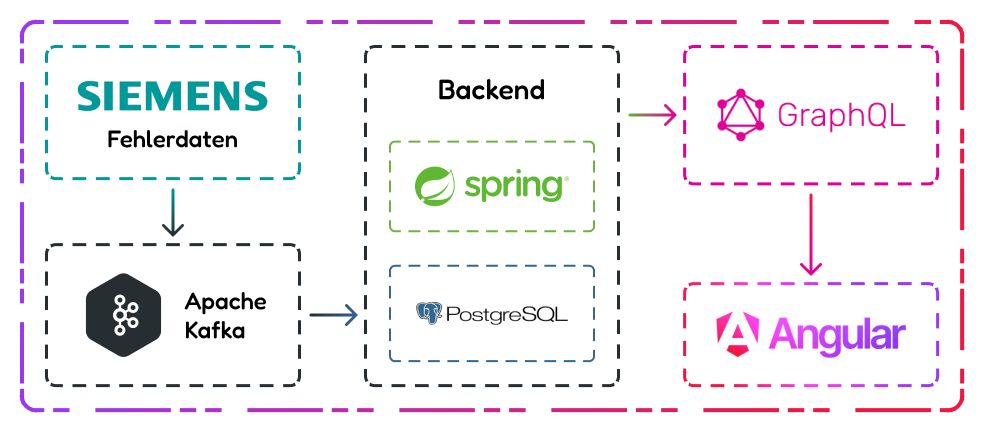
\includegraphics[width=0.8\textwidth]{content/img/Architecture/Architecture.jpg}
    \caption{Diese Darstellung zeigt den schematischen Aufbau der Applikation.}
    \label{fig:architecture_einleitung}
\end{figure}
\FloatBarrier
\section{Initial situation and problem definition}

The company Siemens develops a system called Siemens GNA for many customers both within and outside of Austria, which constantly monitors and guarantees the reliability of the power grid. Due to the numerous elements such as busbars, surge arresters, generators, transformers, disconnectors, circuit breakers, stations, fuses, and load break switches, this utility grid consists of highly complex data. Additionally, with so many elements, it is easy for certain errors, usually in the form of deviations from set values, to occur in the network model. These errors are detected by Siemens, but currently, there is no application available to efficiently process and visualize these collected error data.

Engineers at Siemens analyze the errors using simple text files, which are difficult to read and unnecessarily prolong the duration of repair in the event of a major outage. To make the analysis of error data more efficient, Clemens Schlipfinger and Felix Schneider are developing an application that visualizes these interconnected data with optimal visualization methods. In this work, they focus particularly on the design of a decoupled backend system, which is implemented in the prototype using Apache Kafka, and some suitable visualization methods for such complex data.

As you can see, the illustration \ref{fig:architecture_introduction} visualizes the architecture of our system. First, the fault data is generated by a piece of software from Siemens, which is called GNA (\emph{Global Network Analysis}) and transported to the backend over a fail-safe Apache Kafka system. This message bus decouples our system and the software from Siemens even more and enhances the reliability. Subsequently, the data is saved into a relational database called PostgreSQL. The GraphQL API provides an interface for the frontend application, which is based on the JavaScript-Framework Angular. The frontend offers great visualizations and filters in order to provide intuitive information.

\begin{figure}
    \centering
    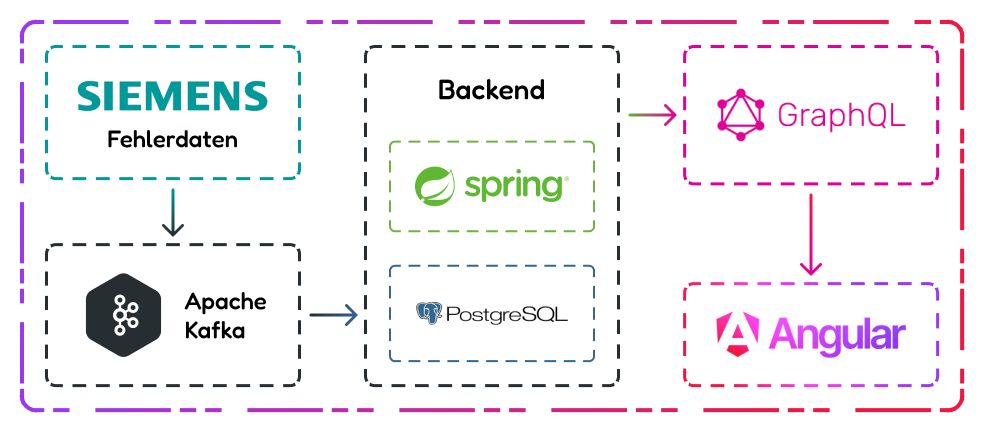
\includegraphics[width=0.8\textwidth]{content/img/Architecture/Architecture.jpg}
    \caption{This illustration shows the architecture of our application.}
    \label{fig:architecture_introduction}
\end{figure}
\FloatBarrier
\section{Forschungsfragen}

\subsection{Message Propagation}

Heutzutage ist die Ausfallsicherheit moderner Systeme von höchster Wichtigkeit. Entkoppelte Systeme fördern die Last, unter welcher Applikationen operieren können. Ein Service ist mit anderen niedrig gekoppelt, wenn wenig Abhängigkeiten gegeben sind. Die Messagepropagation unterstützt ein System dahingehend, die Kommunikation zwischen den einzelnen Softwarekomponenten in ein eigenes Service auszulagern. Welche Form der Messagepropagation am besten für verschiedene Anwendungszwecke geeignet ist, ist demnach eine Frage von hoher Bedeutung.

Demnach wird folgendes Gebiet erforscht:

\textit{Vergleich der verschiedenen Formen der Messagepropagation in Enterprise Service Bus Technologien}

\subsection{Optimale Darstellungsmethoden}

Soziale Netzwerke, biologische Systeme, Nahrungsketten, Dateisysteme und viele weitere Vorkommnisse stark vernetzter Daten verlangen eine effiziente Visualisierung dieser Datenflut. Vernetzungen dieser Art können in den meisten Fällen in gigantischen Graphen dargestellt werden, jedoch können daraus keine Informationen für das Treffen relevanter Entscheidungen getroffen werden. Wie komplexe Daten deswegen intuitiv und verständlich dargestellt werden, ist eine essenzielle Frage bei der Entwicklung solcher Systeme.

Daraus ergibt sich folgende Forschungsfrage:

\textit{Visualisierungsmethoden für stark vernetzte Daten}
\section{Strukturierung der Arbeit}

Der Inhalt dieser Arbeit unterteilt sich in drei Hauptabschnitte. Jedes dieser Kapitel kann eindeutig einem Abschnitt zugeordnet werden. Die Hauptabschnitte beschäftigen sich in erster Linie mit dem Sammeln aller aktuell vorhandenen Informationen zu den jeweiligen Themen, bekannt als \emph{State of the Art} oder \emph{Research}. Um mit der Materie vertraut zu werden, sind bestehende Forschungen der Literatur zusammengetragen und aufgearbeitet worden. Anschließend folgt der empirische Teil mit den Erklärungen der Implementierung des Prototypens, welcher zum Beweisen der These herangezogen wird, und schlussendlich die Bewertung der Forschungsfragen. Letzteres inkludiert einen Katalog zur Bestimmung der richtigen Form von Message Propagation und Vor- und Nachteile der verschiedenen Visualisierungsmethoden bei stark vernetzten Daten.
\chapter{Einleitung}
\label{chp:introduction}
\section{Ausgangssituation und Problemstellung}

Das Unternehmen Siemens entwickelt für viele Kunden innerhalb und außerhalb von Österreich ein System, welches die Ausfallsicherheit des Stromnetzwerkes ständig überprüft und somit garantiert. Diese Software trägt den Namen \emph{Siemens GNA}. Aufgrund der unzähligen Elemente, wie zum Beispiel Sammelschienen, Ableiter, Generatoren, Transformatoren, Trennschalter, Leistungsschalter, Stationen, Sicherungen und Lasttrennschalter, besteht dieses Stromnetzwerk aus äußerst komplexen Daten. Außerdem kann es bei so vielen Elementen leicht passieren, dass gewisse Fehler, meistens in Form von Abweichungen von Sollwerten, im Netzmodell auftreten. Diese Fehler werden von Siemens erfasst, jedoch wird aktuell über keine Applikation verfügt, welche diese gefundenen Fehlerdaten effizient verarbeitet und visualisiert. Die Ingenieure bei Siemens analysieren die Fehler mittels einfachen Textdateien, welche nur schwer lesbar sind und bei einem groben Ausfall die Dauer der Reparatur unnötig vergrößern.

Um die Analyse der Fehlerdaten effizienter zu machen, schreiben Clemens Schlipfinger und Felix Schneider eine Applikation, welche diese stark vernetzten Daten mit optimalen Darstellungsarten visualisiert. Dabei gehen wir in dieser Arbeit besonders auf die Gestaltung eines entkoppelten Backend-Systems und einige geeigneten Visualisierungsarten für solch komplexe Daten ein. 

In der Abbildung \ref{fig:architecture_einleitung} wird die Architektur unserer Applikation zur Fehlervisualisierung dargestellt. Die Fehlerdaten werden von der Siemens GNA Software (\emph{Global Network Analysis} erzeugt und mittels Apache Kafka an das Backend-System übertragen. Damit wird eine hohe Entkoppelung zwischen der Siemens Software und unserem System erreicht. Für die Entwicklung und die Verwaltung von beiden Systemen ist eine hohe Unabhängigkeit von großem Wert. Anschließend werden diese Daten in eine PostgreSQL Datenbank gespeichert und mit einer GraphQL API zur Verfügung gestellt. Das Frontend, welches mit dem JavaScript Framework Angular entwickelt worden ist, wird mit Tabellen und Graphen die Fehler visualisieren.  

\begin{figure}
    \centering
    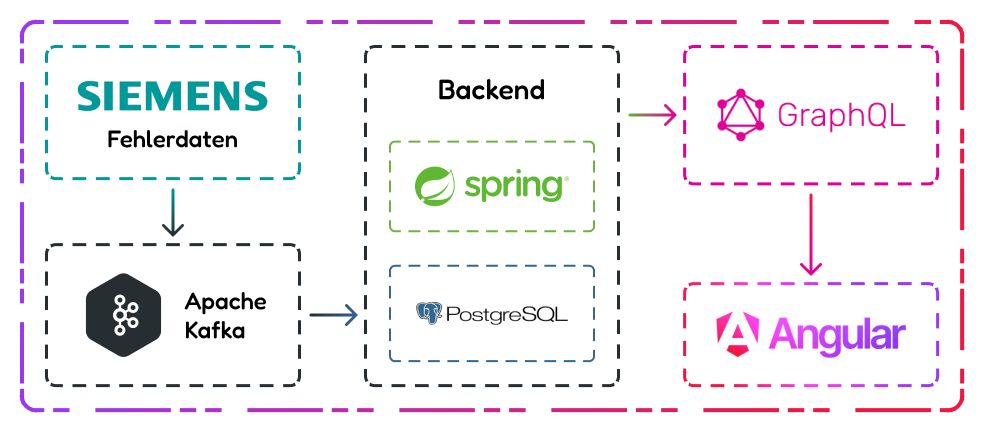
\includegraphics[width=0.8\textwidth]{content/img/Architecture/Architecture.jpg}
    \caption{Diese Darstellung zeigt den schematischen Aufbau der Applikation.}
    \label{fig:architecture_einleitung}
\end{figure}
\FloatBarrier
\section{Initial situation and problem definition}

The company Siemens develops a system called Siemens GNA for many customers both within and outside of Austria, which constantly monitors and guarantees the reliability of the power grid. Due to the numerous elements such as busbars, surge arresters, generators, transformers, disconnectors, circuit breakers, stations, fuses, and load break switches, this utility grid consists of highly complex data. Additionally, with so many elements, it is easy for certain errors, usually in the form of deviations from set values, to occur in the network model. These errors are detected by Siemens, but currently, there is no application available to efficiently process and visualize these collected error data.

Engineers at Siemens analyze the errors using simple text files, which are difficult to read and unnecessarily prolong the duration of repair in the event of a major outage. To make the analysis of error data more efficient, Clemens Schlipfinger and Felix Schneider are developing an application that visualizes these interconnected data with optimal visualization methods. In this work, they focus particularly on the design of a decoupled backend system, which is implemented in the prototype using Apache Kafka, and some suitable visualization methods for such complex data.

As you can see, the illustration \ref{fig:architecture_introduction} visualizes the architecture of our system. First, the fault data is generated by a piece of software from Siemens, which is called GNA (\emph{Global Network Analysis}) and transported to the backend over a fail-safe Apache Kafka system. This message bus decouples our system and the software from Siemens even more and enhances the reliability. Subsequently, the data is saved into a relational database called PostgreSQL. The GraphQL API provides an interface for the frontend application, which is based on the JavaScript-Framework Angular. The frontend offers great visualizations and filters in order to provide intuitive information.

\begin{figure}
    \centering
    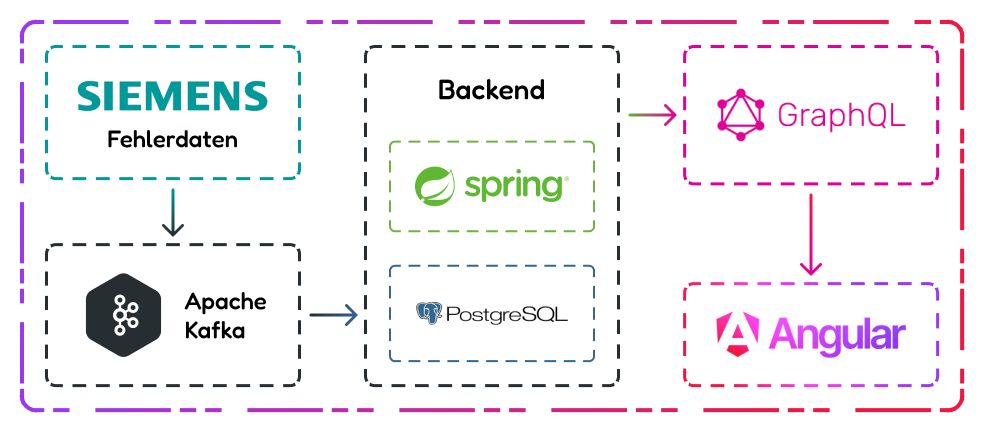
\includegraphics[width=0.8\textwidth]{content/img/Architecture/Architecture.jpg}
    \caption{This illustration shows the architecture of our application.}
    \label{fig:architecture_introduction}
\end{figure}
\FloatBarrier
\section{Forschungsfragen}

\subsection{Message Propagation}

Heutzutage ist die Ausfallsicherheit moderner Systeme von höchster Wichtigkeit. Entkoppelte Systeme fördern die Last, unter welcher Applikationen operieren können. Ein Service ist mit anderen niedrig gekoppelt, wenn wenig Abhängigkeiten gegeben sind. Die Messagepropagation unterstützt ein System dahingehend, die Kommunikation zwischen den einzelnen Softwarekomponenten in ein eigenes Service auszulagern. Welche Form der Messagepropagation am besten für verschiedene Anwendungszwecke geeignet ist, ist demnach eine Frage von hoher Bedeutung.

Demnach wird folgendes Gebiet erforscht:

\textit{Vergleich der verschiedenen Formen der Messagepropagation in Enterprise Service Bus Technologien}

\subsection{Optimale Darstellungsmethoden}

Soziale Netzwerke, biologische Systeme, Nahrungsketten, Dateisysteme und viele weitere Vorkommnisse stark vernetzter Daten verlangen eine effiziente Visualisierung dieser Datenflut. Vernetzungen dieser Art können in den meisten Fällen in gigantischen Graphen dargestellt werden, jedoch können daraus keine Informationen für das Treffen relevanter Entscheidungen getroffen werden. Wie komplexe Daten deswegen intuitiv und verständlich dargestellt werden, ist eine essenzielle Frage bei der Entwicklung solcher Systeme.

Daraus ergibt sich folgende Forschungsfrage:

\textit{Visualisierungsmethoden für stark vernetzte Daten}
\section{Strukturierung der Arbeit}

Der Inhalt dieser Arbeit unterteilt sich in drei Hauptabschnitte. Jedes dieser Kapitel kann eindeutig einem Abschnitt zugeordnet werden. Die Hauptabschnitte beschäftigen sich in erster Linie mit dem Sammeln aller aktuell vorhandenen Informationen zu den jeweiligen Themen, bekannt als \emph{State of the Art} oder \emph{Research}. Um mit der Materie vertraut zu werden, sind bestehende Forschungen der Literatur zusammengetragen und aufgearbeitet worden. Anschließend folgt der empirische Teil mit den Erklärungen der Implementierung des Prototypens, welcher zum Beweisen der These herangezogen wird, und schlussendlich die Bewertung der Forschungsfragen. Letzteres inkludiert einen Katalog zur Bestimmung der richtigen Form von Message Propagation und Vor- und Nachteile der verschiedenen Visualisierungsmethoden bei stark vernetzten Daten.
\chapter{Einleitung}
\label{chp:introduction}
\section{Ausgangssituation und Problemstellung}

Das Unternehmen Siemens entwickelt für viele Kunden innerhalb und außerhalb von Österreich ein System, welches die Ausfallsicherheit des Stromnetzwerkes ständig überprüft und somit garantiert. Diese Software trägt den Namen \emph{Siemens GNA}. Aufgrund der unzähligen Elemente, wie zum Beispiel Sammelschienen, Ableiter, Generatoren, Transformatoren, Trennschalter, Leistungsschalter, Stationen, Sicherungen und Lasttrennschalter, besteht dieses Stromnetzwerk aus äußerst komplexen Daten. Außerdem kann es bei so vielen Elementen leicht passieren, dass gewisse Fehler, meistens in Form von Abweichungen von Sollwerten, im Netzmodell auftreten. Diese Fehler werden von Siemens erfasst, jedoch wird aktuell über keine Applikation verfügt, welche diese gefundenen Fehlerdaten effizient verarbeitet und visualisiert. Die Ingenieure bei Siemens analysieren die Fehler mittels einfachen Textdateien, welche nur schwer lesbar sind und bei einem groben Ausfall die Dauer der Reparatur unnötig vergrößern.

Um die Analyse der Fehlerdaten effizienter zu machen, schreiben Clemens Schlipfinger und Felix Schneider eine Applikation, welche diese stark vernetzten Daten mit optimalen Darstellungsarten visualisiert. Dabei gehen wir in dieser Arbeit besonders auf die Gestaltung eines entkoppelten Backend-Systems und einige geeigneten Visualisierungsarten für solch komplexe Daten ein. 

In der Abbildung \ref{fig:architecture_einleitung} wird die Architektur unserer Applikation zur Fehlervisualisierung dargestellt. Die Fehlerdaten werden von der Siemens GNA Software (\emph{Global Network Analysis} erzeugt und mittels Apache Kafka an das Backend-System übertragen. Damit wird eine hohe Entkoppelung zwischen der Siemens Software und unserem System erreicht. Für die Entwicklung und die Verwaltung von beiden Systemen ist eine hohe Unabhängigkeit von großem Wert. Anschließend werden diese Daten in eine PostgreSQL Datenbank gespeichert und mit einer GraphQL API zur Verfügung gestellt. Das Frontend, welches mit dem JavaScript Framework Angular entwickelt worden ist, wird mit Tabellen und Graphen die Fehler visualisieren.  

\begin{figure}
    \centering
    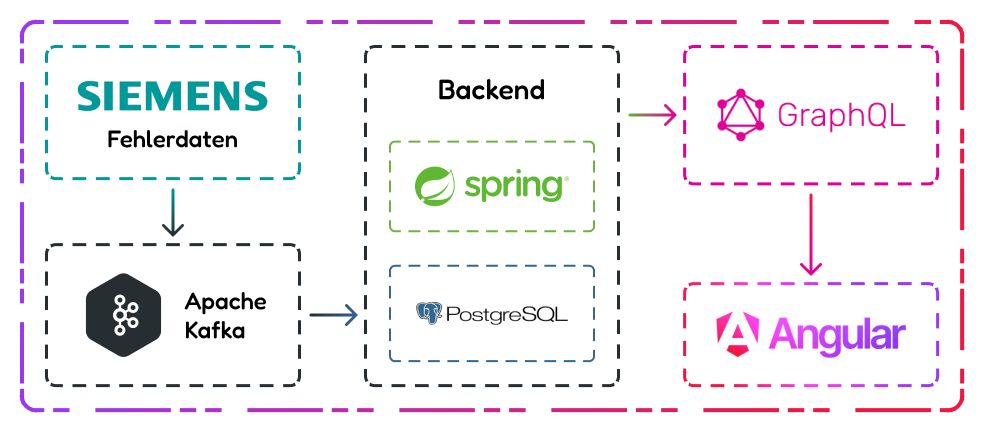
\includegraphics[width=0.8\textwidth]{content/img/Architecture/Architecture.jpg}
    \caption{Diese Darstellung zeigt den schematischen Aufbau der Applikation.}
    \label{fig:architecture_einleitung}
\end{figure}
\FloatBarrier
\section{Initial situation and problem definition}

The company Siemens develops a system called Siemens GNA for many customers both within and outside of Austria, which constantly monitors and guarantees the reliability of the power grid. Due to the numerous elements such as busbars, surge arresters, generators, transformers, disconnectors, circuit breakers, stations, fuses, and load break switches, this utility grid consists of highly complex data. Additionally, with so many elements, it is easy for certain errors, usually in the form of deviations from set values, to occur in the network model. These errors are detected by Siemens, but currently, there is no application available to efficiently process and visualize these collected error data.

Engineers at Siemens analyze the errors using simple text files, which are difficult to read and unnecessarily prolong the duration of repair in the event of a major outage. To make the analysis of error data more efficient, Clemens Schlipfinger and Felix Schneider are developing an application that visualizes these interconnected data with optimal visualization methods. In this work, they focus particularly on the design of a decoupled backend system, which is implemented in the prototype using Apache Kafka, and some suitable visualization methods for such complex data.

As you can see, the illustration \ref{fig:architecture_introduction} visualizes the architecture of our system. First, the fault data is generated by a piece of software from Siemens, which is called GNA (\emph{Global Network Analysis}) and transported to the backend over a fail-safe Apache Kafka system. This message bus decouples our system and the software from Siemens even more and enhances the reliability. Subsequently, the data is saved into a relational database called PostgreSQL. The GraphQL API provides an interface for the frontend application, which is based on the JavaScript-Framework Angular. The frontend offers great visualizations and filters in order to provide intuitive information.

\begin{figure}
    \centering
    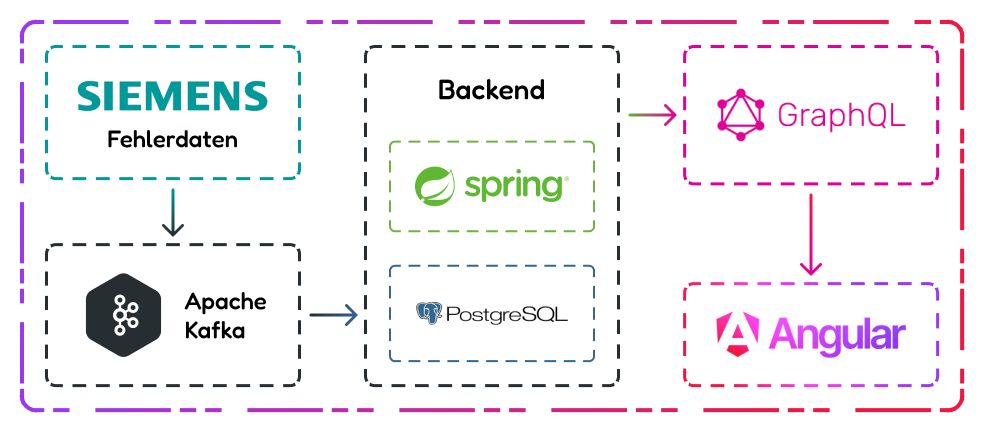
\includegraphics[width=0.8\textwidth]{content/img/Architecture/Architecture.jpg}
    \caption{This illustration shows the architecture of our application.}
    \label{fig:architecture_introduction}
\end{figure}
\FloatBarrier
\section{Forschungsfragen}

\subsection{Message Propagation}

Heutzutage ist die Ausfallsicherheit moderner Systeme von höchster Wichtigkeit. Entkoppelte Systeme fördern die Last, unter welcher Applikationen operieren können. Ein Service ist mit anderen niedrig gekoppelt, wenn wenig Abhängigkeiten gegeben sind. Die Messagepropagation unterstützt ein System dahingehend, die Kommunikation zwischen den einzelnen Softwarekomponenten in ein eigenes Service auszulagern. Welche Form der Messagepropagation am besten für verschiedene Anwendungszwecke geeignet ist, ist demnach eine Frage von hoher Bedeutung.

Demnach wird folgendes Gebiet erforscht:

\textit{Vergleich der verschiedenen Formen der Messagepropagation in Enterprise Service Bus Technologien}

\subsection{Optimale Darstellungsmethoden}

Soziale Netzwerke, biologische Systeme, Nahrungsketten, Dateisysteme und viele weitere Vorkommnisse stark vernetzter Daten verlangen eine effiziente Visualisierung dieser Datenflut. Vernetzungen dieser Art können in den meisten Fällen in gigantischen Graphen dargestellt werden, jedoch können daraus keine Informationen für das Treffen relevanter Entscheidungen getroffen werden. Wie komplexe Daten deswegen intuitiv und verständlich dargestellt werden, ist eine essenzielle Frage bei der Entwicklung solcher Systeme.

Daraus ergibt sich folgende Forschungsfrage:

\textit{Visualisierungsmethoden für stark vernetzte Daten}
\section{Strukturierung der Arbeit}

Der Inhalt dieser Arbeit unterteilt sich in drei Hauptabschnitte. Jedes dieser Kapitel kann eindeutig einem Abschnitt zugeordnet werden. Die Hauptabschnitte beschäftigen sich in erster Linie mit dem Sammeln aller aktuell vorhandenen Informationen zu den jeweiligen Themen, bekannt als \emph{State of the Art} oder \emph{Research}. Um mit der Materie vertraut zu werden, sind bestehende Forschungen der Literatur zusammengetragen und aufgearbeitet worden. Anschließend folgt der empirische Teil mit den Erklärungen der Implementierung des Prototypens, welcher zum Beweisen der These herangezogen wird, und schlussendlich die Bewertung der Forschungsfragen. Letzteres inkludiert einen Katalog zur Bestimmung der richtigen Form von Message Propagation und Vor- und Nachteile der verschiedenen Visualisierungsmethoden bei stark vernetzten Daten.
\chapter{Einleitung}
\label{chp:introduction}
\section{Ausgangssituation und Problemstellung}

Das Unternehmen Siemens entwickelt für viele Kunden innerhalb und außerhalb von Österreich ein System, welches die Ausfallsicherheit des Stromnetzwerkes ständig überprüft und somit garantiert. Diese Software trägt den Namen \emph{Siemens GNA}. Aufgrund der unzähligen Elemente, wie zum Beispiel Sammelschienen, Ableiter, Generatoren, Transformatoren, Trennschalter, Leistungsschalter, Stationen, Sicherungen und Lasttrennschalter, besteht dieses Stromnetzwerk aus äußerst komplexen Daten. Außerdem kann es bei so vielen Elementen leicht passieren, dass gewisse Fehler, meistens in Form von Abweichungen von Sollwerten, im Netzmodell auftreten. Diese Fehler werden von Siemens erfasst, jedoch wird aktuell über keine Applikation verfügt, welche diese gefundenen Fehlerdaten effizient verarbeitet und visualisiert. Die Ingenieure bei Siemens analysieren die Fehler mittels einfachen Textdateien, welche nur schwer lesbar sind und bei einem groben Ausfall die Dauer der Reparatur unnötig vergrößern.

Um die Analyse der Fehlerdaten effizienter zu machen, schreiben Clemens Schlipfinger und Felix Schneider eine Applikation, welche diese stark vernetzten Daten mit optimalen Darstellungsarten visualisiert. Dabei gehen wir in dieser Arbeit besonders auf die Gestaltung eines entkoppelten Backend-Systems und einige geeigneten Visualisierungsarten für solch komplexe Daten ein. 

In der Abbildung \ref{fig:architecture_einleitung} wird die Architektur unserer Applikation zur Fehlervisualisierung dargestellt. Die Fehlerdaten werden von der Siemens GNA Software (\emph{Global Network Analysis} erzeugt und mittels Apache Kafka an das Backend-System übertragen. Damit wird eine hohe Entkoppelung zwischen der Siemens Software und unserem System erreicht. Für die Entwicklung und die Verwaltung von beiden Systemen ist eine hohe Unabhängigkeit von großem Wert. Anschließend werden diese Daten in eine PostgreSQL Datenbank gespeichert und mit einer GraphQL API zur Verfügung gestellt. Das Frontend, welches mit dem JavaScript Framework Angular entwickelt worden ist, wird mit Tabellen und Graphen die Fehler visualisieren.  

\begin{figure}
    \centering
    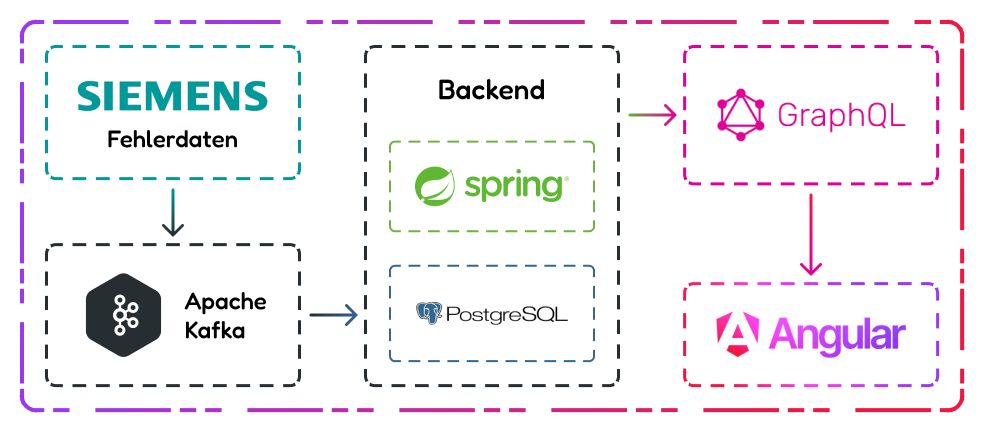
\includegraphics[width=0.8\textwidth]{content/img/Architecture/Architecture.jpg}
    \caption{Diese Darstellung zeigt den schematischen Aufbau der Applikation.}
    \label{fig:architecture_einleitung}
\end{figure}
\FloatBarrier
\section{Initial situation and problem definition}

The company Siemens develops a system called Siemens GNA for many customers both within and outside of Austria, which constantly monitors and guarantees the reliability of the power grid. Due to the numerous elements such as busbars, surge arresters, generators, transformers, disconnectors, circuit breakers, stations, fuses, and load break switches, this utility grid consists of highly complex data. Additionally, with so many elements, it is easy for certain errors, usually in the form of deviations from set values, to occur in the network model. These errors are detected by Siemens, but currently, there is no application available to efficiently process and visualize these collected error data.

Engineers at Siemens analyze the errors using simple text files, which are difficult to read and unnecessarily prolong the duration of repair in the event of a major outage. To make the analysis of error data more efficient, Clemens Schlipfinger and Felix Schneider are developing an application that visualizes these interconnected data with optimal visualization methods. In this work, they focus particularly on the design of a decoupled backend system, which is implemented in the prototype using Apache Kafka, and some suitable visualization methods for such complex data.

As you can see, the illustration \ref{fig:architecture_introduction} visualizes the architecture of our system. First, the fault data is generated by a piece of software from Siemens, which is called GNA (\emph{Global Network Analysis}) and transported to the backend over a fail-safe Apache Kafka system. This message bus decouples our system and the software from Siemens even more and enhances the reliability. Subsequently, the data is saved into a relational database called PostgreSQL. The GraphQL API provides an interface for the frontend application, which is based on the JavaScript-Framework Angular. The frontend offers great visualizations and filters in order to provide intuitive information.

\begin{figure}
    \centering
    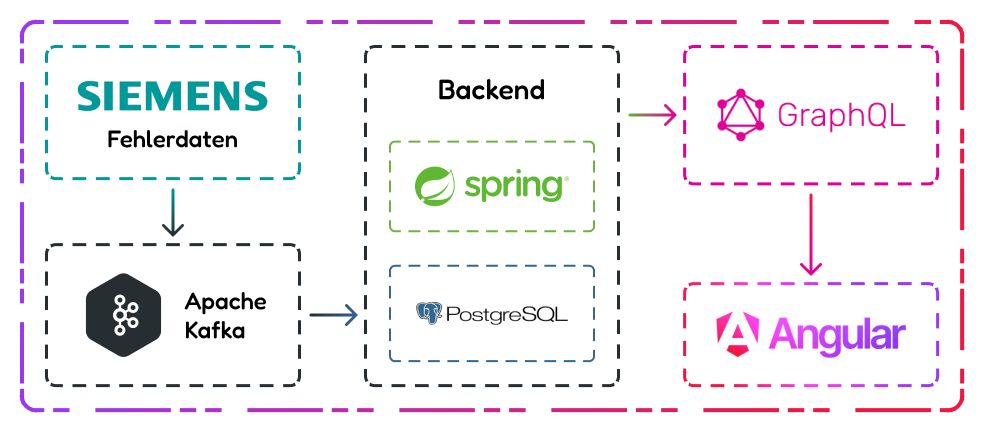
\includegraphics[width=0.8\textwidth]{content/img/Architecture/Architecture.jpg}
    \caption{This illustration shows the architecture of our application.}
    \label{fig:architecture_introduction}
\end{figure}
\FloatBarrier
\section{Forschungsfragen}

\subsection{Message Propagation}

Heutzutage ist die Ausfallsicherheit moderner Systeme von höchster Wichtigkeit. Entkoppelte Systeme fördern die Last, unter welcher Applikationen operieren können. Ein Service ist mit anderen niedrig gekoppelt, wenn wenig Abhängigkeiten gegeben sind. Die Messagepropagation unterstützt ein System dahingehend, die Kommunikation zwischen den einzelnen Softwarekomponenten in ein eigenes Service auszulagern. Welche Form der Messagepropagation am besten für verschiedene Anwendungszwecke geeignet ist, ist demnach eine Frage von hoher Bedeutung.

Demnach wird folgendes Gebiet erforscht:

\textit{Vergleich der verschiedenen Formen der Messagepropagation in Enterprise Service Bus Technologien}

\subsection{Optimale Darstellungsmethoden}

Soziale Netzwerke, biologische Systeme, Nahrungsketten, Dateisysteme und viele weitere Vorkommnisse stark vernetzter Daten verlangen eine effiziente Visualisierung dieser Datenflut. Vernetzungen dieser Art können in den meisten Fällen in gigantischen Graphen dargestellt werden, jedoch können daraus keine Informationen für das Treffen relevanter Entscheidungen getroffen werden. Wie komplexe Daten deswegen intuitiv und verständlich dargestellt werden, ist eine essenzielle Frage bei der Entwicklung solcher Systeme.

Daraus ergibt sich folgende Forschungsfrage:

\textit{Visualisierungsmethoden für stark vernetzte Daten}
\section{Strukturierung der Arbeit}

Der Inhalt dieser Arbeit unterteilt sich in drei Hauptabschnitte. Jedes dieser Kapitel kann eindeutig einem Abschnitt zugeordnet werden. Die Hauptabschnitte beschäftigen sich in erster Linie mit dem Sammeln aller aktuell vorhandenen Informationen zu den jeweiligen Themen, bekannt als \emph{State of the Art} oder \emph{Research}. Um mit der Materie vertraut zu werden, sind bestehende Forschungen der Literatur zusammengetragen und aufgearbeitet worden. Anschließend folgt der empirische Teil mit den Erklärungen der Implementierung des Prototypens, welcher zum Beweisen der These herangezogen wird, und schlussendlich die Bewertung der Forschungsfragen. Letzteres inkludiert einen Katalog zur Bestimmung der richtigen Form von Message Propagation und Vor- und Nachteile der verschiedenen Visualisierungsmethoden bei stark vernetzten Daten.
\chapter{Einleitung}
\label{chp:introduction}
\section{Ausgangssituation und Problemstellung}

Das Unternehmen Siemens entwickelt für viele Kunden innerhalb und außerhalb von Österreich ein System, welches die Ausfallsicherheit des Stromnetzwerkes ständig überprüft und somit garantiert. Diese Software trägt den Namen \emph{Siemens GNA}. Aufgrund der unzähligen Elemente, wie zum Beispiel Sammelschienen, Ableiter, Generatoren, Transformatoren, Trennschalter, Leistungsschalter, Stationen, Sicherungen und Lasttrennschalter, besteht dieses Stromnetzwerk aus äußerst komplexen Daten. Außerdem kann es bei so vielen Elementen leicht passieren, dass gewisse Fehler, meistens in Form von Abweichungen von Sollwerten, im Netzmodell auftreten. Diese Fehler werden von Siemens erfasst, jedoch wird aktuell über keine Applikation verfügt, welche diese gefundenen Fehlerdaten effizient verarbeitet und visualisiert. Die Ingenieure bei Siemens analysieren die Fehler mittels einfachen Textdateien, welche nur schwer lesbar sind und bei einem groben Ausfall die Dauer der Reparatur unnötig vergrößern.

Um die Analyse der Fehlerdaten effizienter zu machen, schreiben Clemens Schlipfinger und Felix Schneider eine Applikation, welche diese stark vernetzten Daten mit optimalen Darstellungsarten visualisiert. Dabei gehen wir in dieser Arbeit besonders auf die Gestaltung eines entkoppelten Backend-Systems und einige geeigneten Visualisierungsarten für solch komplexe Daten ein. 

In der Abbildung \ref{fig:architecture_einleitung} wird die Architektur unserer Applikation zur Fehlervisualisierung dargestellt. Die Fehlerdaten werden von der Siemens GNA Software (\emph{Global Network Analysis} erzeugt und mittels Apache Kafka an das Backend-System übertragen. Damit wird eine hohe Entkoppelung zwischen der Siemens Software und unserem System erreicht. Für die Entwicklung und die Verwaltung von beiden Systemen ist eine hohe Unabhängigkeit von großem Wert. Anschließend werden diese Daten in eine PostgreSQL Datenbank gespeichert und mit einer GraphQL API zur Verfügung gestellt. Das Frontend, welches mit dem JavaScript Framework Angular entwickelt worden ist, wird mit Tabellen und Graphen die Fehler visualisieren.  

\begin{figure}
    \centering
    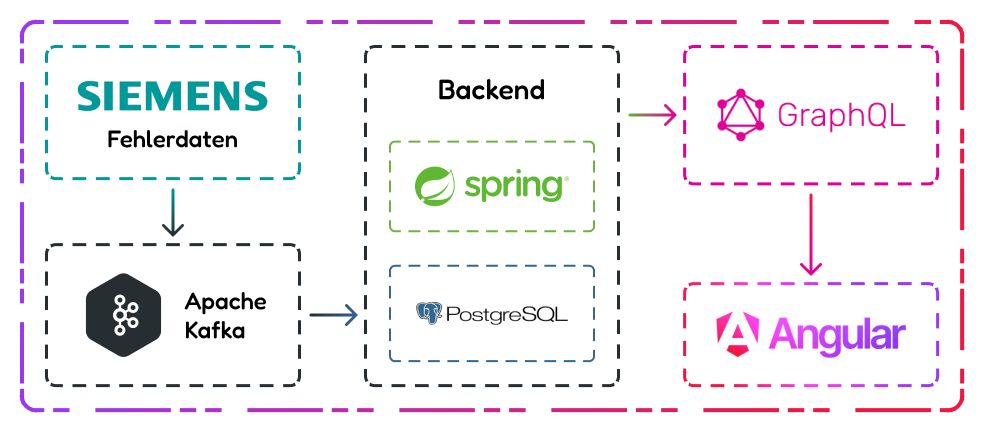
\includegraphics[width=0.8\textwidth]{content/img/Architecture/Architecture.jpg}
    \caption{Diese Darstellung zeigt den schematischen Aufbau der Applikation.}
    \label{fig:architecture_einleitung}
\end{figure}
\FloatBarrier
\section{Initial situation and problem definition}

The company Siemens develops a system called Siemens GNA for many customers both within and outside of Austria, which constantly monitors and guarantees the reliability of the power grid. Due to the numerous elements such as busbars, surge arresters, generators, transformers, disconnectors, circuit breakers, stations, fuses, and load break switches, this utility grid consists of highly complex data. Additionally, with so many elements, it is easy for certain errors, usually in the form of deviations from set values, to occur in the network model. These errors are detected by Siemens, but currently, there is no application available to efficiently process and visualize these collected error data.

Engineers at Siemens analyze the errors using simple text files, which are difficult to read and unnecessarily prolong the duration of repair in the event of a major outage. To make the analysis of error data more efficient, Clemens Schlipfinger and Felix Schneider are developing an application that visualizes these interconnected data with optimal visualization methods. In this work, they focus particularly on the design of a decoupled backend system, which is implemented in the prototype using Apache Kafka, and some suitable visualization methods for such complex data.

As you can see, the illustration \ref{fig:architecture_introduction} visualizes the architecture of our system. First, the fault data is generated by a piece of software from Siemens, which is called GNA (\emph{Global Network Analysis}) and transported to the backend over a fail-safe Apache Kafka system. This message bus decouples our system and the software from Siemens even more and enhances the reliability. Subsequently, the data is saved into a relational database called PostgreSQL. The GraphQL API provides an interface for the frontend application, which is based on the JavaScript-Framework Angular. The frontend offers great visualizations and filters in order to provide intuitive information.

\begin{figure}
    \centering
    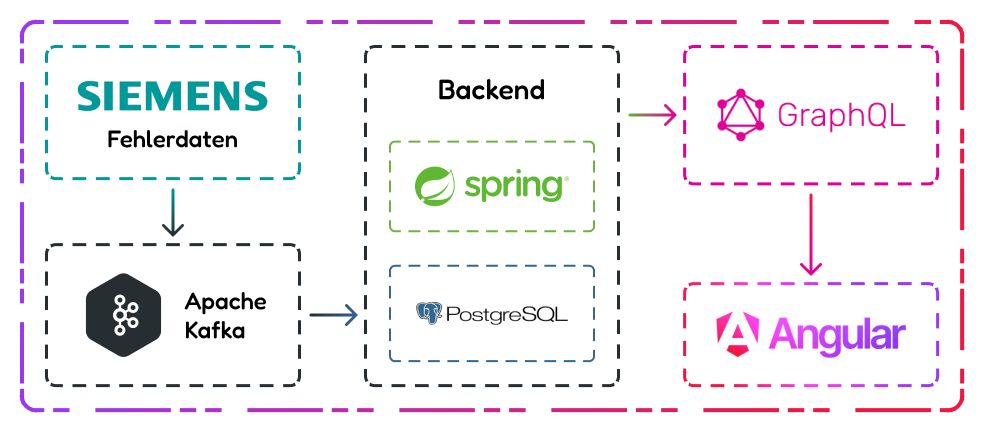
\includegraphics[width=0.8\textwidth]{content/img/Architecture/Architecture.jpg}
    \caption{This illustration shows the architecture of our application.}
    \label{fig:architecture_introduction}
\end{figure}
\FloatBarrier
\section{Forschungsfragen}

\subsection{Message Propagation}

Heutzutage ist die Ausfallsicherheit moderner Systeme von höchster Wichtigkeit. Entkoppelte Systeme fördern die Last, unter welcher Applikationen operieren können. Ein Service ist mit anderen niedrig gekoppelt, wenn wenig Abhängigkeiten gegeben sind. Die Messagepropagation unterstützt ein System dahingehend, die Kommunikation zwischen den einzelnen Softwarekomponenten in ein eigenes Service auszulagern. Welche Form der Messagepropagation am besten für verschiedene Anwendungszwecke geeignet ist, ist demnach eine Frage von hoher Bedeutung.

Demnach wird folgendes Gebiet erforscht:

\textit{Vergleich der verschiedenen Formen der Messagepropagation in Enterprise Service Bus Technologien}

\subsection{Optimale Darstellungsmethoden}

Soziale Netzwerke, biologische Systeme, Nahrungsketten, Dateisysteme und viele weitere Vorkommnisse stark vernetzter Daten verlangen eine effiziente Visualisierung dieser Datenflut. Vernetzungen dieser Art können in den meisten Fällen in gigantischen Graphen dargestellt werden, jedoch können daraus keine Informationen für das Treffen relevanter Entscheidungen getroffen werden. Wie komplexe Daten deswegen intuitiv und verständlich dargestellt werden, ist eine essenzielle Frage bei der Entwicklung solcher Systeme.

Daraus ergibt sich folgende Forschungsfrage:

\textit{Visualisierungsmethoden für stark vernetzte Daten}
\section{Strukturierung der Arbeit}

Der Inhalt dieser Arbeit unterteilt sich in drei Hauptabschnitte. Jedes dieser Kapitel kann eindeutig einem Abschnitt zugeordnet werden. Die Hauptabschnitte beschäftigen sich in erster Linie mit dem Sammeln aller aktuell vorhandenen Informationen zu den jeweiligen Themen, bekannt als \emph{State of the Art} oder \emph{Research}. Um mit der Materie vertraut zu werden, sind bestehende Forschungen der Literatur zusammengetragen und aufgearbeitet worden. Anschließend folgt der empirische Teil mit den Erklärungen der Implementierung des Prototypens, welcher zum Beweisen der These herangezogen wird, und schlussendlich die Bewertung der Forschungsfragen. Letzteres inkludiert einen Katalog zur Bestimmung der richtigen Form von Message Propagation und Vor- und Nachteile der verschiedenen Visualisierungsmethoden bei stark vernetzten Daten.
\chapter{Einleitung}
\label{chp:introduction}
\section{Ausgangssituation und Problemstellung}

Das Unternehmen Siemens entwickelt für viele Kunden innerhalb und außerhalb von Österreich ein System, welches die Ausfallsicherheit des Stromnetzwerkes ständig überprüft und somit garantiert. Diese Software trägt den Namen \emph{Siemens GNA}. Aufgrund der unzähligen Elemente, wie zum Beispiel Sammelschienen, Ableiter, Generatoren, Transformatoren, Trennschalter, Leistungsschalter, Stationen, Sicherungen und Lasttrennschalter, besteht dieses Stromnetzwerk aus äußerst komplexen Daten. Außerdem kann es bei so vielen Elementen leicht passieren, dass gewisse Fehler, meistens in Form von Abweichungen von Sollwerten, im Netzmodell auftreten. Diese Fehler werden von Siemens erfasst, jedoch wird aktuell über keine Applikation verfügt, welche diese gefundenen Fehlerdaten effizient verarbeitet und visualisiert. Die Ingenieure bei Siemens analysieren die Fehler mittels einfachen Textdateien, welche nur schwer lesbar sind und bei einem groben Ausfall die Dauer der Reparatur unnötig vergrößern.

Um die Analyse der Fehlerdaten effizienter zu machen, schreiben Clemens Schlipfinger und Felix Schneider eine Applikation, welche diese stark vernetzten Daten mit optimalen Darstellungsarten visualisiert. Dabei gehen wir in dieser Arbeit besonders auf die Gestaltung eines entkoppelten Backend-Systems und einige geeigneten Visualisierungsarten für solch komplexe Daten ein. 

In der Abbildung \ref{fig:architecture_einleitung} wird die Architektur unserer Applikation zur Fehlervisualisierung dargestellt. Die Fehlerdaten werden von der Siemens GNA Software (\emph{Global Network Analysis} erzeugt und mittels Apache Kafka an das Backend-System übertragen. Damit wird eine hohe Entkoppelung zwischen der Siemens Software und unserem System erreicht. Für die Entwicklung und die Verwaltung von beiden Systemen ist eine hohe Unabhängigkeit von großem Wert. Anschließend werden diese Daten in eine PostgreSQL Datenbank gespeichert und mit einer GraphQL API zur Verfügung gestellt. Das Frontend, welches mit dem JavaScript Framework Angular entwickelt worden ist, wird mit Tabellen und Graphen die Fehler visualisieren.  

\begin{figure}
    \centering
    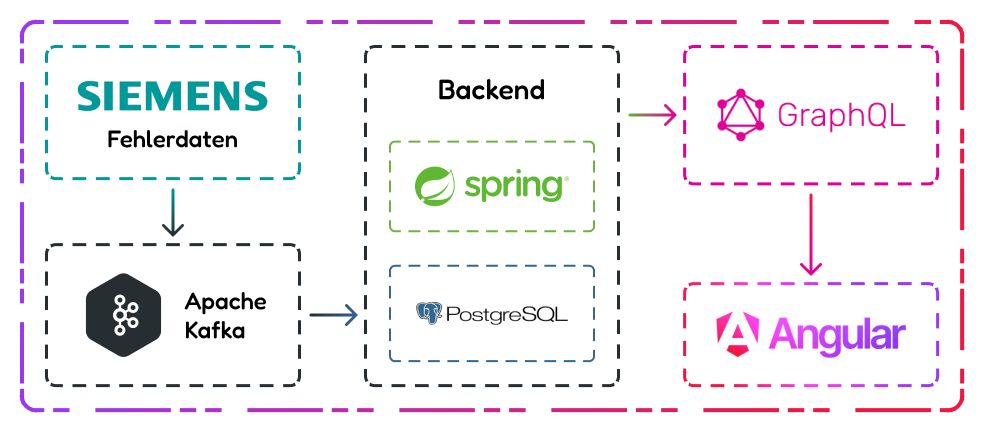
\includegraphics[width=0.8\textwidth]{content/img/Architecture/Architecture.jpg}
    \caption{Diese Darstellung zeigt den schematischen Aufbau der Applikation.}
    \label{fig:architecture_einleitung}
\end{figure}
\FloatBarrier
\section{Initial situation and problem definition}

The company Siemens develops a system called Siemens GNA for many customers both within and outside of Austria, which constantly monitors and guarantees the reliability of the power grid. Due to the numerous elements such as busbars, surge arresters, generators, transformers, disconnectors, circuit breakers, stations, fuses, and load break switches, this utility grid consists of highly complex data. Additionally, with so many elements, it is easy for certain errors, usually in the form of deviations from set values, to occur in the network model. These errors are detected by Siemens, but currently, there is no application available to efficiently process and visualize these collected error data.

Engineers at Siemens analyze the errors using simple text files, which are difficult to read and unnecessarily prolong the duration of repair in the event of a major outage. To make the analysis of error data more efficient, Clemens Schlipfinger and Felix Schneider are developing an application that visualizes these interconnected data with optimal visualization methods. In this work, they focus particularly on the design of a decoupled backend system, which is implemented in the prototype using Apache Kafka, and some suitable visualization methods for such complex data.

As you can see, the illustration \ref{fig:architecture_introduction} visualizes the architecture of our system. First, the fault data is generated by a piece of software from Siemens, which is called GNA (\emph{Global Network Analysis}) and transported to the backend over a fail-safe Apache Kafka system. This message bus decouples our system and the software from Siemens even more and enhances the reliability. Subsequently, the data is saved into a relational database called PostgreSQL. The GraphQL API provides an interface for the frontend application, which is based on the JavaScript-Framework Angular. The frontend offers great visualizations and filters in order to provide intuitive information.

\begin{figure}
    \centering
    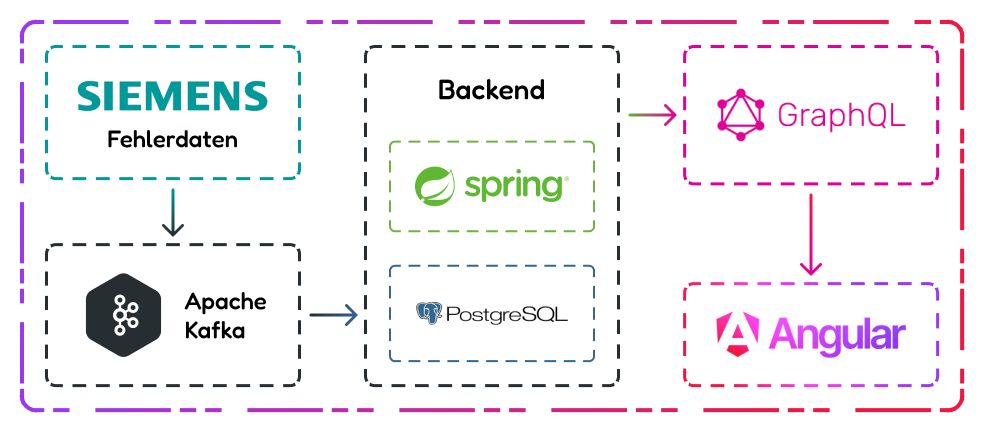
\includegraphics[width=0.8\textwidth]{content/img/Architecture/Architecture.jpg}
    \caption{This illustration shows the architecture of our application.}
    \label{fig:architecture_introduction}
\end{figure}
\FloatBarrier
\section{Forschungsfragen}

\subsection{Message Propagation}

Heutzutage ist die Ausfallsicherheit moderner Systeme von höchster Wichtigkeit. Entkoppelte Systeme fördern die Last, unter welcher Applikationen operieren können. Ein Service ist mit anderen niedrig gekoppelt, wenn wenig Abhängigkeiten gegeben sind. Die Messagepropagation unterstützt ein System dahingehend, die Kommunikation zwischen den einzelnen Softwarekomponenten in ein eigenes Service auszulagern. Welche Form der Messagepropagation am besten für verschiedene Anwendungszwecke geeignet ist, ist demnach eine Frage von hoher Bedeutung.

Demnach wird folgendes Gebiet erforscht:

\textit{Vergleich der verschiedenen Formen der Messagepropagation in Enterprise Service Bus Technologien}

\subsection{Optimale Darstellungsmethoden}

Soziale Netzwerke, biologische Systeme, Nahrungsketten, Dateisysteme und viele weitere Vorkommnisse stark vernetzter Daten verlangen eine effiziente Visualisierung dieser Datenflut. Vernetzungen dieser Art können in den meisten Fällen in gigantischen Graphen dargestellt werden, jedoch können daraus keine Informationen für das Treffen relevanter Entscheidungen getroffen werden. Wie komplexe Daten deswegen intuitiv und verständlich dargestellt werden, ist eine essenzielle Frage bei der Entwicklung solcher Systeme.

Daraus ergibt sich folgende Forschungsfrage:

\textit{Visualisierungsmethoden für stark vernetzte Daten}
\section{Strukturierung der Arbeit}

Der Inhalt dieser Arbeit unterteilt sich in drei Hauptabschnitte. Jedes dieser Kapitel kann eindeutig einem Abschnitt zugeordnet werden. Die Hauptabschnitte beschäftigen sich in erster Linie mit dem Sammeln aller aktuell vorhandenen Informationen zu den jeweiligen Themen, bekannt als \emph{State of the Art} oder \emph{Research}. Um mit der Materie vertraut zu werden, sind bestehende Forschungen der Literatur zusammengetragen und aufgearbeitet worden. Anschließend folgt der empirische Teil mit den Erklärungen der Implementierung des Prototypens, welcher zum Beweisen der These herangezogen wird, und schlussendlich die Bewertung der Forschungsfragen. Letzteres inkludiert einen Katalog zur Bestimmung der richtigen Form von Message Propagation und Vor- und Nachteile der verschiedenen Visualisierungsmethoden bei stark vernetzten Daten.
\chapter{Einleitung}
\label{chp:introduction}
\section{Ausgangssituation und Problemstellung}

Das Unternehmen Siemens entwickelt für viele Kunden innerhalb und außerhalb von Österreich ein System, welches die Ausfallsicherheit des Stromnetzwerkes ständig überprüft und somit garantiert. Diese Software trägt den Namen \emph{Siemens GNA}. Aufgrund der unzähligen Elemente, wie zum Beispiel Sammelschienen, Ableiter, Generatoren, Transformatoren, Trennschalter, Leistungsschalter, Stationen, Sicherungen und Lasttrennschalter, besteht dieses Stromnetzwerk aus äußerst komplexen Daten. Außerdem kann es bei so vielen Elementen leicht passieren, dass gewisse Fehler, meistens in Form von Abweichungen von Sollwerten, im Netzmodell auftreten. Diese Fehler werden von Siemens erfasst, jedoch wird aktuell über keine Applikation verfügt, welche diese gefundenen Fehlerdaten effizient verarbeitet und visualisiert. Die Ingenieure bei Siemens analysieren die Fehler mittels einfachen Textdateien, welche nur schwer lesbar sind und bei einem groben Ausfall die Dauer der Reparatur unnötig vergrößern.

Um die Analyse der Fehlerdaten effizienter zu machen, schreiben Clemens Schlipfinger und Felix Schneider eine Applikation, welche diese stark vernetzten Daten mit optimalen Darstellungsarten visualisiert. Dabei gehen wir in dieser Arbeit besonders auf die Gestaltung eines entkoppelten Backend-Systems und einige geeigneten Visualisierungsarten für solch komplexe Daten ein. 

In der Abbildung \ref{fig:architecture_einleitung} wird die Architektur unserer Applikation zur Fehlervisualisierung dargestellt. Die Fehlerdaten werden von der Siemens GNA Software (\emph{Global Network Analysis} erzeugt und mittels Apache Kafka an das Backend-System übertragen. Damit wird eine hohe Entkoppelung zwischen der Siemens Software und unserem System erreicht. Für die Entwicklung und die Verwaltung von beiden Systemen ist eine hohe Unabhängigkeit von großem Wert. Anschließend werden diese Daten in eine PostgreSQL Datenbank gespeichert und mit einer GraphQL API zur Verfügung gestellt. Das Frontend, welches mit dem JavaScript Framework Angular entwickelt worden ist, wird mit Tabellen und Graphen die Fehler visualisieren.  

\begin{figure}
    \centering
    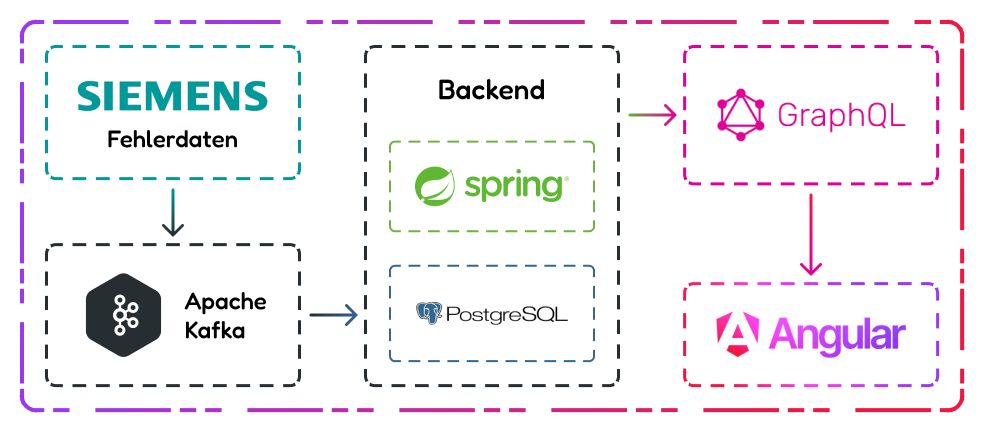
\includegraphics[width=0.8\textwidth]{content/img/Architecture/Architecture.jpg}
    \caption{Diese Darstellung zeigt den schematischen Aufbau der Applikation.}
    \label{fig:architecture_einleitung}
\end{figure}
\FloatBarrier
\section{Initial situation and problem definition}

The company Siemens develops a system called Siemens GNA for many customers both within and outside of Austria, which constantly monitors and guarantees the reliability of the power grid. Due to the numerous elements such as busbars, surge arresters, generators, transformers, disconnectors, circuit breakers, stations, fuses, and load break switches, this utility grid consists of highly complex data. Additionally, with so many elements, it is easy for certain errors, usually in the form of deviations from set values, to occur in the network model. These errors are detected by Siemens, but currently, there is no application available to efficiently process and visualize these collected error data.

Engineers at Siemens analyze the errors using simple text files, which are difficult to read and unnecessarily prolong the duration of repair in the event of a major outage. To make the analysis of error data more efficient, Clemens Schlipfinger and Felix Schneider are developing an application that visualizes these interconnected data with optimal visualization methods. In this work, they focus particularly on the design of a decoupled backend system, which is implemented in the prototype using Apache Kafka, and some suitable visualization methods for such complex data.

As you can see, the illustration \ref{fig:architecture_introduction} visualizes the architecture of our system. First, the fault data is generated by a piece of software from Siemens, which is called GNA (\emph{Global Network Analysis}) and transported to the backend over a fail-safe Apache Kafka system. This message bus decouples our system and the software from Siemens even more and enhances the reliability. Subsequently, the data is saved into a relational database called PostgreSQL. The GraphQL API provides an interface for the frontend application, which is based on the JavaScript-Framework Angular. The frontend offers great visualizations and filters in order to provide intuitive information.

\begin{figure}
    \centering
    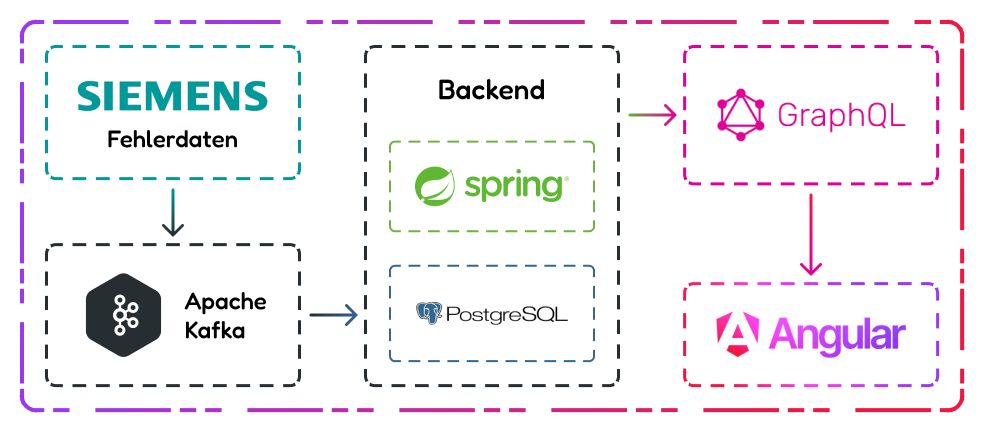
\includegraphics[width=0.8\textwidth]{content/img/Architecture/Architecture.jpg}
    \caption{This illustration shows the architecture of our application.}
    \label{fig:architecture_introduction}
\end{figure}
\FloatBarrier
\section{Forschungsfragen}

\subsection{Message Propagation}

Heutzutage ist die Ausfallsicherheit moderner Systeme von höchster Wichtigkeit. Entkoppelte Systeme fördern die Last, unter welcher Applikationen operieren können. Ein Service ist mit anderen niedrig gekoppelt, wenn wenig Abhängigkeiten gegeben sind. Die Messagepropagation unterstützt ein System dahingehend, die Kommunikation zwischen den einzelnen Softwarekomponenten in ein eigenes Service auszulagern. Welche Form der Messagepropagation am besten für verschiedene Anwendungszwecke geeignet ist, ist demnach eine Frage von hoher Bedeutung.

Demnach wird folgendes Gebiet erforscht:

\textit{Vergleich der verschiedenen Formen der Messagepropagation in Enterprise Service Bus Technologien}

\subsection{Optimale Darstellungsmethoden}

Soziale Netzwerke, biologische Systeme, Nahrungsketten, Dateisysteme und viele weitere Vorkommnisse stark vernetzter Daten verlangen eine effiziente Visualisierung dieser Datenflut. Vernetzungen dieser Art können in den meisten Fällen in gigantischen Graphen dargestellt werden, jedoch können daraus keine Informationen für das Treffen relevanter Entscheidungen getroffen werden. Wie komplexe Daten deswegen intuitiv und verständlich dargestellt werden, ist eine essenzielle Frage bei der Entwicklung solcher Systeme.

Daraus ergibt sich folgende Forschungsfrage:

\textit{Visualisierungsmethoden für stark vernetzte Daten}
\section{Strukturierung der Arbeit}

Der Inhalt dieser Arbeit unterteilt sich in drei Hauptabschnitte. Jedes dieser Kapitel kann eindeutig einem Abschnitt zugeordnet werden. Die Hauptabschnitte beschäftigen sich in erster Linie mit dem Sammeln aller aktuell vorhandenen Informationen zu den jeweiligen Themen, bekannt als \emph{State of the Art} oder \emph{Research}. Um mit der Materie vertraut zu werden, sind bestehende Forschungen der Literatur zusammengetragen und aufgearbeitet worden. Anschließend folgt der empirische Teil mit den Erklärungen der Implementierung des Prototypens, welcher zum Beweisen der These herangezogen wird, und schlussendlich die Bewertung der Forschungsfragen. Letzteres inkludiert einen Katalog zur Bestimmung der richtigen Form von Message Propagation und Vor- und Nachteile der verschiedenen Visualisierungsmethoden bei stark vernetzten Daten.
%Roemische Nummerierung im Inhaltsverzeichnis
\renewcommand\thechapter{\Roman{chapter}} 
%Beginnen der Roemischen Nummerierung bei I
\setcounter{chapter}{0} 
%bindet Literatur-, Abbildungs-, Tabellenverzeichnis ein
%
% Literatur-, Abbildungs-, Tabellen- und Abkuerzungsverzeichnis
%


% Literaturverzeichnis ===>>>> siehe DA.bib
\nocite{*} %alle Einträge aus DA.bib werden übernommen, auch diese, die nicht im Text vorkommen
\bibliographystyle{babunsrt} %sortiere Verzeichnis nach Reihenfolge im Text
\bibliography{DA} %erstelle Verzeichnis

% erstellt ein File mit der Liste aller Bilder (Endung: *.lof)
\listoffigures

% erstellt ein File mit der Liste aller Tabellen (Endung: *.lot)
\listoftables

\renewcommand\lstlistlistingname{Quellcodeverzeichnis} 
\lstlistoflistings 

\chapter{Abk\"urzungsverzeichnis}

\vspace{3mm}

\textbf{AMQP} Advanced Message Queuing Protocol -- Ein offenes Netzwerkprotokoll zum Verwaltung von Nachrichten zwischen Anwendungen.

\vspace{5mm}

\textbf{API} Application Programming Interface -- Eine Schnittstelle, die es Anwendungen ermöglicht, miteinander zu kommunizieren und auf bestimmte Funktionen oder Dienste zuzugreifen.

\vspace{5mm}

\textbf{DNS} Domain Name System -- Ein System zur Umwandlung von Domainnamen in IP-Adressen, das für die Navigation im Internet verwendet wird.

\vspace{5mm}

\textbf{HTTP} Hypertext Transfer Protocol -- Ein Protokoll zur Übertragung von Daten über das Internet, das zur Übertragung von Webseiten, Bildern, Videos und anderen Ressourcen verwendet wird.

\vspace{5mm}

\textbf{REST} Representational State Transfer -- Ein Prinzip beziehungsweise Regeln, welche das Internet konzeptionell als eine Sammlung von zustandlosen Ressourcen ansieht und diese als Repräsentationen über Endpunkte zur Verfügung stellt.

\vspace{5mm}

\textbf{SOA} Service-Oriented Architecture -- Ein Architekturstil, der die Erstellung von Anwendungen aus unabhängigen, wiederverwendbaren Diensten betont, die über ein Netzwerk miteinander kommunizieren.

\vspace{5mm}

\textbf{STOMP} Streaming Text Oriented Messaging Protocol -- Ein Protokoll zur Nachrichtenübertragung über Netzwerke, das auf der Idee des Nachrichten-Brokers basiert.

\vspace{5mm}

\textbf{UI} User Interface -- Die Schnittstelle, über die ein Benutzer mit einem Computer oder einer Software interagiert.

\vspace{5mm}

\textbf{UX} User Experience -- Die Gesamtheit der Eindrücke und Emotionen eines Benutzers bei der Interaktion mit einem Produkt oder einer Dienstleistung.

\vspace{5mm}

\textbf{XMPP} Extensible Messaging and Presence Protocol -- Ein offenes Protokoll zur Nachrichtenübertragung und Anwesenheitsinformationen in Echtzeit. Es wird oft für Instant Messaging verwendet.

\renewcommand\thechapter{\Alph{chapter}}
\setcounter{chapter}{0} 
\chapter{Einleitung}
\label{chp:introduction}
\section{Ausgangssituation und Problemstellung}

Das Unternehmen Siemens entwickelt für viele Kunden innerhalb und außerhalb von Österreich ein System, welches die Ausfallsicherheit des Stromnetzwerkes ständig überprüft und somit garantiert. Diese Software trägt den Namen \emph{Siemens GNA}. Aufgrund der unzähligen Elemente, wie zum Beispiel Sammelschienen, Ableiter, Generatoren, Transformatoren, Trennschalter, Leistungsschalter, Stationen, Sicherungen und Lasttrennschalter, besteht dieses Stromnetzwerk aus äußerst komplexen Daten. Außerdem kann es bei so vielen Elementen leicht passieren, dass gewisse Fehler, meistens in Form von Abweichungen von Sollwerten, im Netzmodell auftreten. Diese Fehler werden von Siemens erfasst, jedoch wird aktuell über keine Applikation verfügt, welche diese gefundenen Fehlerdaten effizient verarbeitet und visualisiert. Die Ingenieure bei Siemens analysieren die Fehler mittels einfachen Textdateien, welche nur schwer lesbar sind und bei einem groben Ausfall die Dauer der Reparatur unnötig vergrößern.

Um die Analyse der Fehlerdaten effizienter zu machen, schreiben Clemens Schlipfinger und Felix Schneider eine Applikation, welche diese stark vernetzten Daten mit optimalen Darstellungsarten visualisiert. Dabei gehen wir in dieser Arbeit besonders auf die Gestaltung eines entkoppelten Backend-Systems und einige geeigneten Visualisierungsarten für solch komplexe Daten ein. 

In der Abbildung \ref{fig:architecture_einleitung} wird die Architektur unserer Applikation zur Fehlervisualisierung dargestellt. Die Fehlerdaten werden von der Siemens GNA Software (\emph{Global Network Analysis} erzeugt und mittels Apache Kafka an das Backend-System übertragen. Damit wird eine hohe Entkoppelung zwischen der Siemens Software und unserem System erreicht. Für die Entwicklung und die Verwaltung von beiden Systemen ist eine hohe Unabhängigkeit von großem Wert. Anschließend werden diese Daten in eine PostgreSQL Datenbank gespeichert und mit einer GraphQL API zur Verfügung gestellt. Das Frontend, welches mit dem JavaScript Framework Angular entwickelt worden ist, wird mit Tabellen und Graphen die Fehler visualisieren.  

\begin{figure}
    \centering
    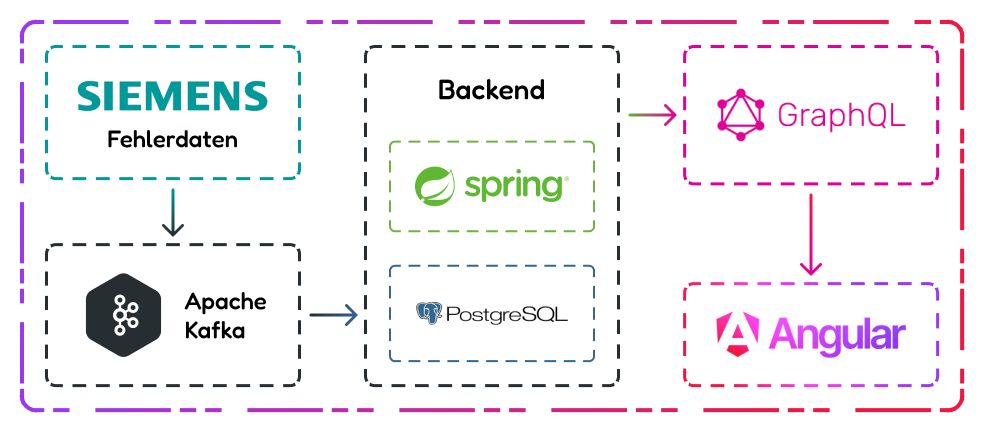
\includegraphics[width=0.8\textwidth]{content/img/Architecture/Architecture.jpg}
    \caption{Diese Darstellung zeigt den schematischen Aufbau der Applikation.}
    \label{fig:architecture_einleitung}
\end{figure}
\FloatBarrier
\section{Initial situation and problem definition}

The company Siemens develops a system called Siemens GNA for many customers both within and outside of Austria, which constantly monitors and guarantees the reliability of the power grid. Due to the numerous elements such as busbars, surge arresters, generators, transformers, disconnectors, circuit breakers, stations, fuses, and load break switches, this utility grid consists of highly complex data. Additionally, with so many elements, it is easy for certain errors, usually in the form of deviations from set values, to occur in the network model. These errors are detected by Siemens, but currently, there is no application available to efficiently process and visualize these collected error data.

Engineers at Siemens analyze the errors using simple text files, which are difficult to read and unnecessarily prolong the duration of repair in the event of a major outage. To make the analysis of error data more efficient, Clemens Schlipfinger and Felix Schneider are developing an application that visualizes these interconnected data with optimal visualization methods. In this work, they focus particularly on the design of a decoupled backend system, which is implemented in the prototype using Apache Kafka, and some suitable visualization methods for such complex data.

As you can see, the illustration \ref{fig:architecture_introduction} visualizes the architecture of our system. First, the fault data is generated by a piece of software from Siemens, which is called GNA (\emph{Global Network Analysis}) and transported to the backend over a fail-safe Apache Kafka system. This message bus decouples our system and the software from Siemens even more and enhances the reliability. Subsequently, the data is saved into a relational database called PostgreSQL. The GraphQL API provides an interface for the frontend application, which is based on the JavaScript-Framework Angular. The frontend offers great visualizations and filters in order to provide intuitive information.

\begin{figure}
    \centering
    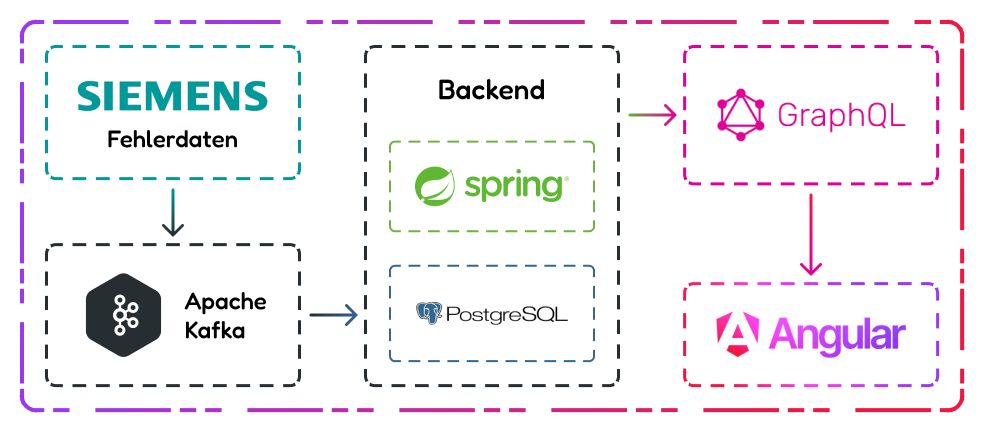
\includegraphics[width=0.8\textwidth]{content/img/Architecture/Architecture.jpg}
    \caption{This illustration shows the architecture of our application.}
    \label{fig:architecture_introduction}
\end{figure}
\FloatBarrier
\section{Forschungsfragen}

\subsection{Message Propagation}

Heutzutage ist die Ausfallsicherheit moderner Systeme von höchster Wichtigkeit. Entkoppelte Systeme fördern die Last, unter welcher Applikationen operieren können. Ein Service ist mit anderen niedrig gekoppelt, wenn wenig Abhängigkeiten gegeben sind. Die Messagepropagation unterstützt ein System dahingehend, die Kommunikation zwischen den einzelnen Softwarekomponenten in ein eigenes Service auszulagern. Welche Form der Messagepropagation am besten für verschiedene Anwendungszwecke geeignet ist, ist demnach eine Frage von hoher Bedeutung.

Demnach wird folgendes Gebiet erforscht:

\textit{Vergleich der verschiedenen Formen der Messagepropagation in Enterprise Service Bus Technologien}

\subsection{Optimale Darstellungsmethoden}

Soziale Netzwerke, biologische Systeme, Nahrungsketten, Dateisysteme und viele weitere Vorkommnisse stark vernetzter Daten verlangen eine effiziente Visualisierung dieser Datenflut. Vernetzungen dieser Art können in den meisten Fällen in gigantischen Graphen dargestellt werden, jedoch können daraus keine Informationen für das Treffen relevanter Entscheidungen getroffen werden. Wie komplexe Daten deswegen intuitiv und verständlich dargestellt werden, ist eine essenzielle Frage bei der Entwicklung solcher Systeme.

Daraus ergibt sich folgende Forschungsfrage:

\textit{Visualisierungsmethoden für stark vernetzte Daten}
\section{Strukturierung der Arbeit}

Der Inhalt dieser Arbeit unterteilt sich in drei Hauptabschnitte. Jedes dieser Kapitel kann eindeutig einem Abschnitt zugeordnet werden. Die Hauptabschnitte beschäftigen sich in erster Linie mit dem Sammeln aller aktuell vorhandenen Informationen zu den jeweiligen Themen, bekannt als \emph{State of the Art} oder \emph{Research}. Um mit der Materie vertraut zu werden, sind bestehende Forschungen der Literatur zusammengetragen und aufgearbeitet worden. Anschließend folgt der empirische Teil mit den Erklärungen der Implementierung des Prototypens, welcher zum Beweisen der These herangezogen wird, und schlussendlich die Bewertung der Forschungsfragen. Letzteres inkludiert einen Katalog zur Bestimmung der richtigen Form von Message Propagation und Vor- und Nachteile der verschiedenen Visualisierungsmethoden bei stark vernetzten Daten.
\end{document}
